\documentclass[12pt,a4paper,openright,twoside]{book}
\usepackage[utf8]{inputenc}

%\newcommand{\thesislang}{italian} % decommentare in caso di tesi in italiano
\newcommand{\thesislang}{english} % commentare in caso di tesi in italiano
\usepackage{thesis-style}

% version
\newcommand{\versionmajor}{0}
\newcommand{\versionminor}{1}
\newcommand{\versionpatch}{2}
\newcommand{\version}{\versionmajor.\versionminor.\versionpatch}
\typeout{Document version: \version}


% For tables
\usepackage{multirow}
\usepackage{longtable}
%\def\arraystretch{1.5}%  1 is the default vertical padding

\begin{document}
	
    %----------------------------------------------------------------------------------------
    % FRONTMATTER
    \frontmatter
    
    % ! TeX root = thesis-main.tex
\title{Master Thesis - Igor Lirussi}
\author{Lirussi Igor}
\date{\today}

\newgeometry{margin=0.8in}
\begin{titlepage}
	\begin{center}
		% \vspace*{0.2cm}
		
		\large
		\textbf{ALMA MATER STUDIORUM -- UNIVERSITY OF BOLOGNA \\ CESENA CAMPUS }
		\\
		\noindent\hrulefill
		\vspace{0.4cm}
		
		\Large
		School of Engineering and Architecture \\
		Second Cycle Degree/Two-year Master in \\Computer Science and Engineering
		
		\Huge
		\vspace{4cm}
		\textbf{
			Novel robotic skill synthesis 
			\\
			with Conditional Neural 
			\\
                Movement Primitives
		}
		
		\large
		\vspace{1cm}
		Master's thesis in 
		\\
		\textsc{Intelligent Robotic Systems}
		
		\vspace{5.5cm}
		\begin{minipage}[t]{0.64\textwidth}
			\begin{flushleft}
				\textit{Supervisor} 
				\\ 
				\textbf{Prof.} \textbf{Andrea Roli}
				\\
				\vspace{0.4cm}
				\textit{Co-Supervisor} 
				\\
				\textbf{Prof.} \textbf{Emre Uğur} \\(Boğaziçi University, Istanbul)
			\end{flushleft}
		\end{minipage}
		\begin{minipage}[t]{0.34\textwidth}
			\begin{flushright}
				\textit{Candidate} 
				\\ 
				\textbf{Igor Lirussi}
			\end{flushright}
		\end{minipage}\\
		
		\vfill
		\noindent\hrulefill
		\vspace{0.3cm}
		\Large
		

		Academic Year 2022-2023
	\end{center}
\end{titlepage}
\restoregeometry

    
    %Max 2000 characters, strict.
\begin{abstract}	

Max 2000 characters, strict. UniBo has that limit in the upload system! Will write at the end.  
\end{abstract}
    
    \begin{dedication} 
    To my family and to the time we have.
    \end{dedication}
    
    % Optional. Max 1 page.
\begin{acknowledgements}
Acknowledgments here. 
% First of all, I would like to thank my advisors, Prof. Emre Uğur and Prof. Andrea Roli, for their support and passion during this intense journey.
% I extend my gratitude to all members of \href{https://colors.cmpe.boun.edu.tr}{CoLoRs Laboratory} in Boğaziçi University for their guidance and kindness. 
% I am grateful to my foreign friends, Bahadir, Naz, and Ipek, for their moral and logistical help abroad. 
% I thank, as well, my Italian friends for their affection, which enables me to explore distant lands far away from home. 
% Finally, I want to express my deepest gratitude to my family. I have been able to persevere in my education thanks to their unconditional love and support.
\end{acknowledgements}
    
    \tableofcontents   
    \listoffigures     
    \listoftables
    % LIST OF SYMBOLS PAGE
\begin{symbols}

% The title will be typeset as "LIST OF SYMBOLS".
% Use a separate \sym command for each symbols definition.
% First, Latin symbols in alphabetical order
\sym{$t$}{Time}
\sym{$r$}{Representation}
\sym{$x$}{Target point (query point) }
\sym{$SM(t)$}{Sensorimotor data at time t}
\sym{$E$}{Encoder network}
\sym{$Q$}{Decoder network}
\sym{$O$}{Set of observation points (conditioning points)}
\sym{$D$}{Set of demonstration trajectories (expert demonstrations)}
\sym{$T$}{Set of target points $x$ desired}
% 1 EMPTY LINE BETWEEN LATIN AND GREEK SYMBOLS GROUP!!!
\sym{}{}
% Then Greek symbols in alphabetical order
\sym{$\alpha$}{Blending parameter \textit{or} scale}
\sym{$\beta_t(i)$}{Backward variable}
\sym{$\gamma$}{External parameter (Task parameter) (TP)}
\sym{$\theta$}{Parameter set of Decoder Network}
\sym{$\phi$}{Parameter set of Encoder Network}
\sym{$\sigma$}{Standard Deviation}
\sym{$\mu$}{Mean}
\sym{$\tau$}{Trajectory}


\end{symbols}
    % LIST OF ABBREV PAGE
\begin{abbreviations}

 % Abbreviations in alphabetical order
\sym{1D}{One Dimensional}
\sym{2D}{Two Dimensional}
\sym{3D}{Three Dimensional}
\sym{IR}{Infrared}
\sym{ROS}{Robot Operating System}
\sym{RGB}{Red Green Blue}
\sym{RGBD}{Red Green Blue Depth}
\sym{SL}{Supervised Learning}
\sym{LfD}{Learning from Demonstration}
\sym{ML}{Machine Learning}
\sym{DL}{Deep Learnign}
\sym{GMM}{Gaussian Mixture Model}
\sym{HMM}{Hidden Markov Model}
\sym{MSE}{Mean Squared Error}
\sym{ReLU}{Rectified Linear Unit}
\sym{GP}{Gaussian Processes}
\sym{NP}{Neural Processes}
\sym{CNP}{Conditional Neural Processes}
\sym{DNP}{Dynamic Movement Primitives}
\sym{Pro-MP}{Probabilistic Movement Primitives}
\sym{CNMP}{Conditional Neural Movement Primitives}
\sym{TP}{Task Parameter}
\sym{YOLO}{You Only Look Once model}
\sym{UR10}{Universal Robot 10}
\sym{DOF}{Degrees of freedom}
\sym{IMU}{Inertial measurement unit}
\sym{RPC}{Remote Procedure Call}
\sym{CPU}{Central Processing Unit}
\sym{GPU}{Graphic Processing Unit}

\end{abbreviations}
    \lstlistoflistings 
    %----------------------------------------------------------------------------------------
    
    \mainmatter
    
    %----------------------------------------------------------------------------------------
\chapter{Introduction}
\label{chap:introduction}
%----------------------------------------------------------------------------------------

\section{Overview}
Humans have been building sequences of actions to achieve 
decision-making under uncertainty, which is essential for achieving high-level goals

In this study, we propose a computational model that is biologically inspired. Our approach 
Implement it on an anthropomorphic robot and on an industrial collaborative robot.
Specifically, ... 

\section{Challanges}
Robotics dominates many fields, but often the environment is controlled, designed to help the robot in it's task and not human friendly. All environments in which humans are present are nor organized nor predictable 
Some jobs have been substituted by machines but are specific and repetitive. Closest contact consumer public with automation is with machines that have a single skill. Vacuum robot can only vacuum, and it's its only capability, dishwasher can only wash dishes, dough mixer does only
\section{Objectives}
 combine not only movement one after the other (end-to-end) but combine parts of them

\section{Thesis Structure} 
Accordingly, the remainder of this thesis is structured as follows.
\Cref{chap:background} discusses the background of the topic, the current advancements in the field, and the related research with a literature review. 
In \cref{chap:platforms} the instruments and frameworks used in this research are listed and analyzed to be able to understand the initial setup and replicate the results. 
The \cref{chap:design} explains the design and architecture of the proposed method. In order to understand the logic, the conceptual passages and mathematical background. 
The \cref{chap:implementation} analyzes the key points of the implemented solution through the explanation of the most important passages in the code developed.
The \cref{chap:validation} shows the final results and the testing on real-life robotic platforms.
Finally, \Cref{chap:conclusions} concludes this thesis by summarising its main contribution and future work.
    %----------------------------------------------------------------------------------------
\chapter{Related Work} % or Background
\label{chap:background}
%----------------------------------------------------------------------------------------

% intro 
In this chapter, we will proceed with the literature analysis and state-of-the-art methods related to the topic. Furthermore, some basic notions regarding the previous research relied upon will be explained.

Trajectory generation for robotics is a topic closely related to manipulation and navigation. Every movement can be described as a trajectory, defined as the composition of the path taken by an agent (or its joints) in time \cite{biagiotti2008trajectory}. 
In this discussion, we will focus more on the manipulation part, being the most clear example of how combining different trajectories can produce novel robotic skills. Manipulation is one of the most distinctive capabilities of robots, since their main objective is to perform physical tasks in the real world. Any process that presents the necessity of a human to engage with a physical object meaningfully can solely be automated by robot manipulation. \cite{rosen2022role}

Creating robots capable of directly interacting with the world around them is still a key challenge in robotics, and manipulation is central to this. \cite{kroemer2021review} 
Nevertheless, the ability to solve high-level goals in robots is increasing \cite{gupta2019relay}, \cite{simeonov2021long} thanks to the recent advances in artificial intelligence.  
Some approaches may follow natural language instructions to achieve complex sequences of actions \cite{hu2019hierarchical}, but according to the research objective, a certain degree of autonomy is desired. This implies typically giving only the final goal and not the step-by-step instructions. 

% some proposals
% Initial approaches utilized ... TODO
% latest proposals


% importance of Learning by Demonstration
A commonly used technique in robotics is Learning from Demonstration (LfD) \cite{ARGALL2009469}, and then \cite{ravichandar2020recent}. It allows for solving a wide variety of robotics problems by imitating an external agent. The demonstrator, often a human or another system, provides examples (expert demonstrations) of how to perform a task, and the learning agent generalizes from these demonstrations to acquire the ability to perform the task later independently.

Famous learning from demonstration research includes statistical modeling \cite{calinon2016tutorial}, dynamic systems \cite{schaal2006dynamic}, and their union in \cite{ugur2020compliant}. In Dynamic Movement Primitives (DMPs) \cite{schaal2006dynamic}, a trajectory is represented with a set of differential equations and learned with as little as one shot. Thanks to the "point attractor" mechanism, it guarantees reaching a point even under perturbations. DMPs have successfully been utilized in difficult manipulation tasks such as in-hand manipulation and flipping boxes using chopsticks \cite{pastor2009learning}. On the other hand, DMPs require additional tuning to determine the number of basis functions. Moreover, their approach is not designed to learn from multiple trajectories and, therefore, cannot encode the important parts of multiple demonstrations \cite{Ugur-RSS-19}. 

In the Probabilistic Movement Primitives (ProMP) \cite{paraschos2013probabilistic}, instead, the distribution of basis functions is often represented using a probabilistic framework, typically a Gaussian Mixture Model (GMM) or a similar probabilistic model. Historically, Gaussian Mixture Models \cite{nguyen2009model} have been prominent among various probabilistic approaches since they provide adaptable solutions to the challenge of modeling trajectories. On the other hand, GMMs involve estimating many parameters, especially when dealing with high-dimensional data or a large number of components. This can make training and inference computationally expensive, particularly when the dataset is extensive, and if not done correctly, can lead to some failures, Figure \ref{fig:prompcnmp}.
\begin{figure}
	\centering
	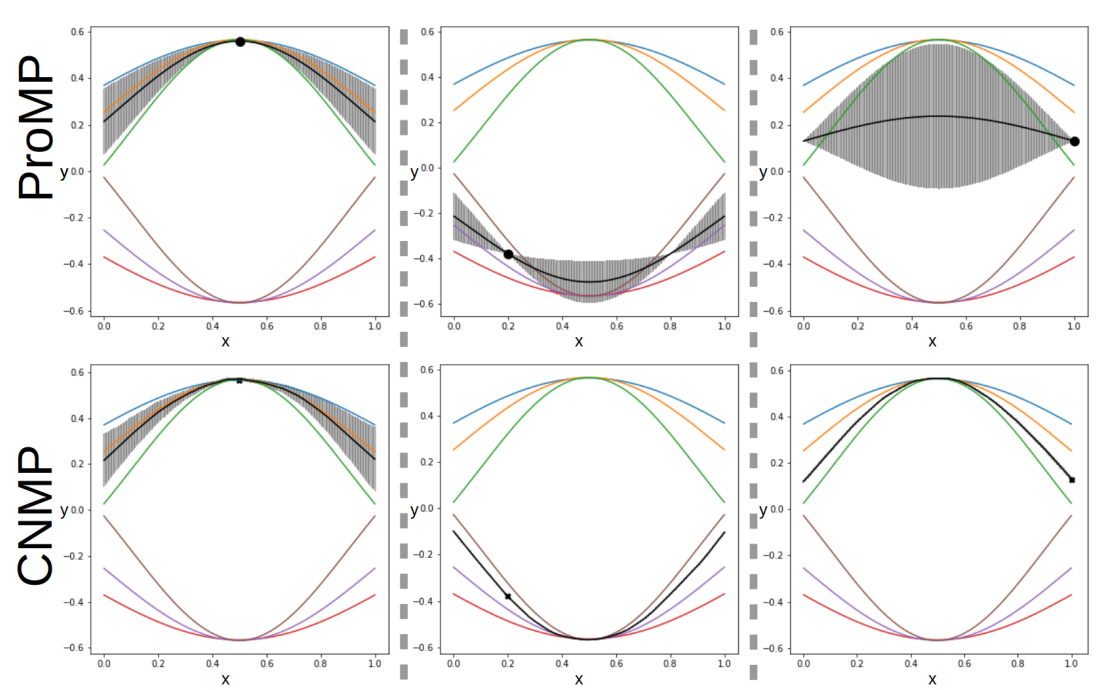
\includegraphics[width=0.5\linewidth]{Images/ProMPvsCNMP.png}
	\caption{In ProMPs the distribution of basis functions is often represented using a probabilistic framework, but can lead to some failures.}
	\label{fig:prompcnmp}
\end{figure}

Another probabilistic model, like GMMs, often used in statistical modeling techniques is Hidden Markov Models (HMMs) \cite{lee2011incremental}. HMMs were successfully applied to learn multi-modal models from temperature, pressure, and fingertip information for exploratory object classification tasks \cite{chu2013using}.

A recent model developed in robotics called Conditional Neural Movement Primitives (CNMP) \cite{Ugur-RSS-19} also learns from demonstrations, but instead of using GMMs, they use neural networks to model the mapping from conditions to trajectories directly. Neural networks allow the model to scale better and to offer robust data approximation via gradient descent. Until recently, neural networks in deep learning were trained to approximate a single-output function. However, when data is a distribution, the single function cannot approximate the underlying model. So the network can be modeled as a probabilistic approximator, that can predict the distribution parameters, mean, and variance. This makes CNMPs well-suited for tasks with complex, high-dimensional state spaces. It allows one to learn skills in tens, rather than thousands, of real-world interactions and interpolate among them.

% our proposal/contribution
Based on the above-mentioned observations, the proposal is as follows.
In the following research, the ability of CNMPs to interpolate the trajectories demonstrated is exploited to synthesize new complex skills. 
The model is based on Gaussian Processes (GP) \cite{seeger2004gaussian}, Neural Processes (NPs) \cite{garnelo2018neural}, and  Conditional Neural Processes (CNPs) \cite{DBLP:journals/corr/abs-1807-01613}.
For context, an explanation in detail of these above-mentioned methods will follow.



%%%%%%% BACKGROUND IN DEPTH %%%%%%%
%%%%%%% GP %%%%%%%
\section{Gaussian Processes}
Gaussian Processes \cite{seeger2004gaussian} are probabilistic models that define a distribution over functions, Figure \ref{fig:gp}.
This means that they leverage pre-existing knowledge about a set of functions and infer during test-time specific functions that fit the data provided. Given a set of observed points, there are infinite possible functions that pass through them. Gaussian processes provide an elegant solution to this challenge by assigning a probability to each of these potential functions. The mean of this probability distribution then represents the most probable characterization of the data given the observation points \cite{Goertler2018VisualExplorationGaussian}. 

This is called regression and is used, for example, in robotics or time series forecasting. Gaussian processes are not limited to regression, and they can also be extended to classification and clustering tasks \cite{kapoor2010gaussian} \cite{kim2007clustering}. 
\begin{figure}
	\centering
	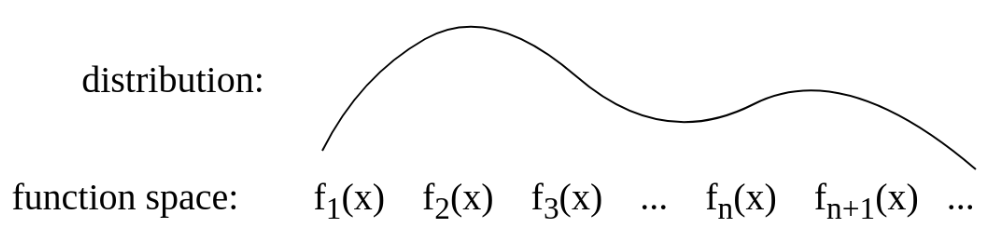
\includegraphics[width=0.9\linewidth]{Images/GP.png}
	\caption{Gaussian Processes are probabilistic models that define a distribution over functions.}
	\label{fig:gp}
\end{figure}
Many supervised learning problems can be seen as function approximations since a dataset of observations $ \{x_i, y_i\}^{n-1}_{i=0}$ is basically a number $n$ of evaluations $y_i = f(x_i)$ of an unknown function $f$. A supervised learning algorithm returns an approximated function $g$. The goal is to minimize the loss between the real function $f$ and the predicted one $g$. The evaluation is carried out on unlabelled data points $x_j$.

On the other hand, the disadvantages of Gaussian Processes are prior selection and training time for large datasets. Scaling issues with GPs have been addressed in \cite{snelson2006sparse}. The limited expressivity from functional restriction was addressed with DeepGPs in \cite{damianou2013deep}  \cite{salimbeni2017doubly}. Overcoming these issues and attempting to combine Deep Learning (DL) with GPs was proposed in \cite{wilson2016deep}, but the approach remains close to GPs since the network is used to learn more expressive kernels to use with GPs.

%%%%%%% CNP %%%%%%%
\section{Conditional Neural Processes}
In \cite{DBLP:journals/corr/abs-1807-01613}, the authors propose a novel research in which the inference potential of Gaussian Processes and the performance of neural networks are blended together. Neural networks are extensively employed as approximators of functions and have demonstrated considerable efficacy but often require large datasets for training. In CNPs, the prior knowledge is directly derived from the data, allowing them to infer the underlying function distribution based on observations. CNPs are built with three main blocks: Encoder, Aggregator, and Decoder. Encoder $E$ and Decoder $Q$ are typically Multi-layer perceptrons. The model structure is shown in Figure \ref{fig:cnp}. 
\begin{figure}
	\centering
	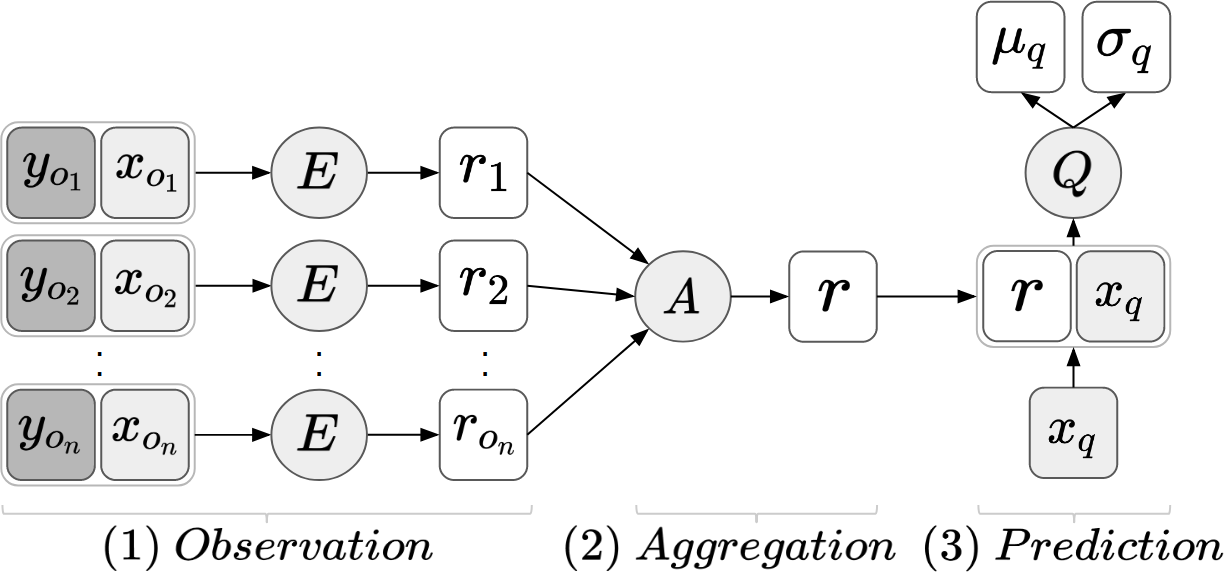
\includegraphics[width=0.5\linewidth]{Images/CNP.png}
	\caption{The structure of a CNP network, with three main blocks: Encoder, Aggregator, and Decoder.}
	\label{fig:cnp}
\end{figure}
The model scales with complexity $O(n+m)$ for making $m$ predictions from $n$ observations, while GPs scale with $O(n+m)^3$. CNPs don't require the specification of a kernel cause they learn it from the data provided in training. The tradeoff is that the representations of the observations have fixed dimensionality.

The work is based on the previous research of Neural Processes (NPs) \cite{garnelo2018neural}. NPs are suggested as a means to manage the substantial computational demands of GPs while leveraging their flexibility and efficiency with data. NPs help create different predictions by learning a shared hidden representation. However, they have trouble with long sequences because they automatically pick certain points. Building on NPs, Conditional Neural Processes (CNPs) are strong models that make training more efficient by allowing explicit conditioning.
\begin{figure}
	\centering
	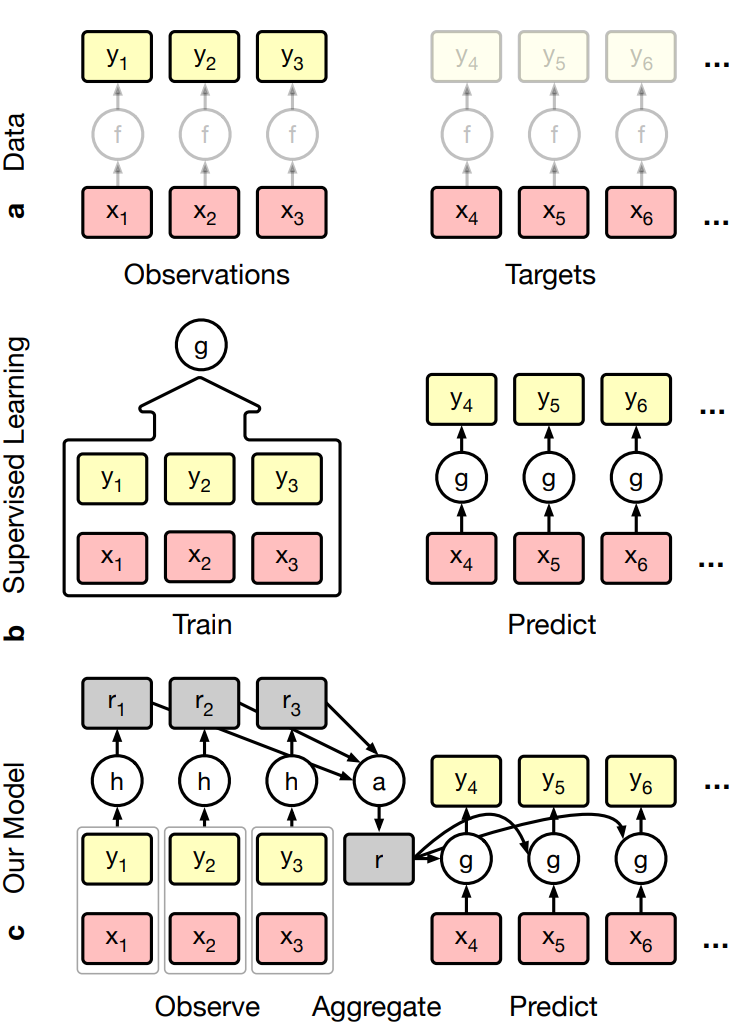
\includegraphics[width=0.5\linewidth]{Images/CNPdata.png}
	\caption{CNP allows precise predictions for targets sampled from a distribution conditioned with observations}
	\label{fig:cnp_data}
\end{figure}
The approach allows precise predictions for targets sampled from a distribution conditioned with observations, Figure \ref{fig:cnp_data}. Given a varying number of observations $O$, a neural network $E$ is utilized as an encoder to generate a fixed-size representation $r_i$.

Observations fed to the network don't have an order, following the stochastic processes, because subsequently, they are aggregated with the average operation to obtain a single representation $r$. Any commutative operation is valid and usable. The resulting representation $r$ contains the conditioning information and is fed to a decoder network $Q$ along with the desired target $x_j$ to query. The decoder network $Q$ has parameters $\theta$. For all the targets $x_j \in T$ the decoder outputs the mean and standard deviation.

The formulation of the encoding of each observation is:
\begin{equation}
r_i = E_\phi(x_i,y_i), \quad \forall(x_i,y_i) \in O
\end{equation}
and the following commutative operation between the encodings to create a single one: 
\begin{equation}
    r = r_1 \oplus r_2 \oplus ... \oplus r_i,
\end{equation}
The commutative operation expressed by $\oplus$, can be summation, average, product, and so on. 

The vector generated is concatenated with the target variables. The merged representation is passed to the decoder to obtain the output as:
\begin{equation}
    \phi_j = Q_\theta(x_j, r), \quad \forall x_j \in T
\end{equation}
Where the output is: 
\begin{equation}
    \phi_j = (\mu_j, \sigma_j^2)
\end{equation}
which are the mean and the standard deviation of the output variable.

In summary, the CNP model, with averaging operation, can be formulated as: 
\begin{equation}
    \mu_j, \sigma_j^2 = Q_\theta \left( x_j \oplus \frac{ \sum_{i}^{n} E\phi((x_i,y_i)) }{n}  \right)
\end{equation}

%%%%%%% CNMP %%%%%%%
\section{Conditional Neural Movement Primitives}
Finally, in \cite{Ugur-RSS-19}, Conditional Neural Movement Primitives are proposed as a model. CNMPs, as the name suggests, are an extension of CNPs and are particularly well suited for the robotics domain. The model illustration can be seen in Figure \ref{fig:cnmp}.  
\begin{figure}
	\centering
	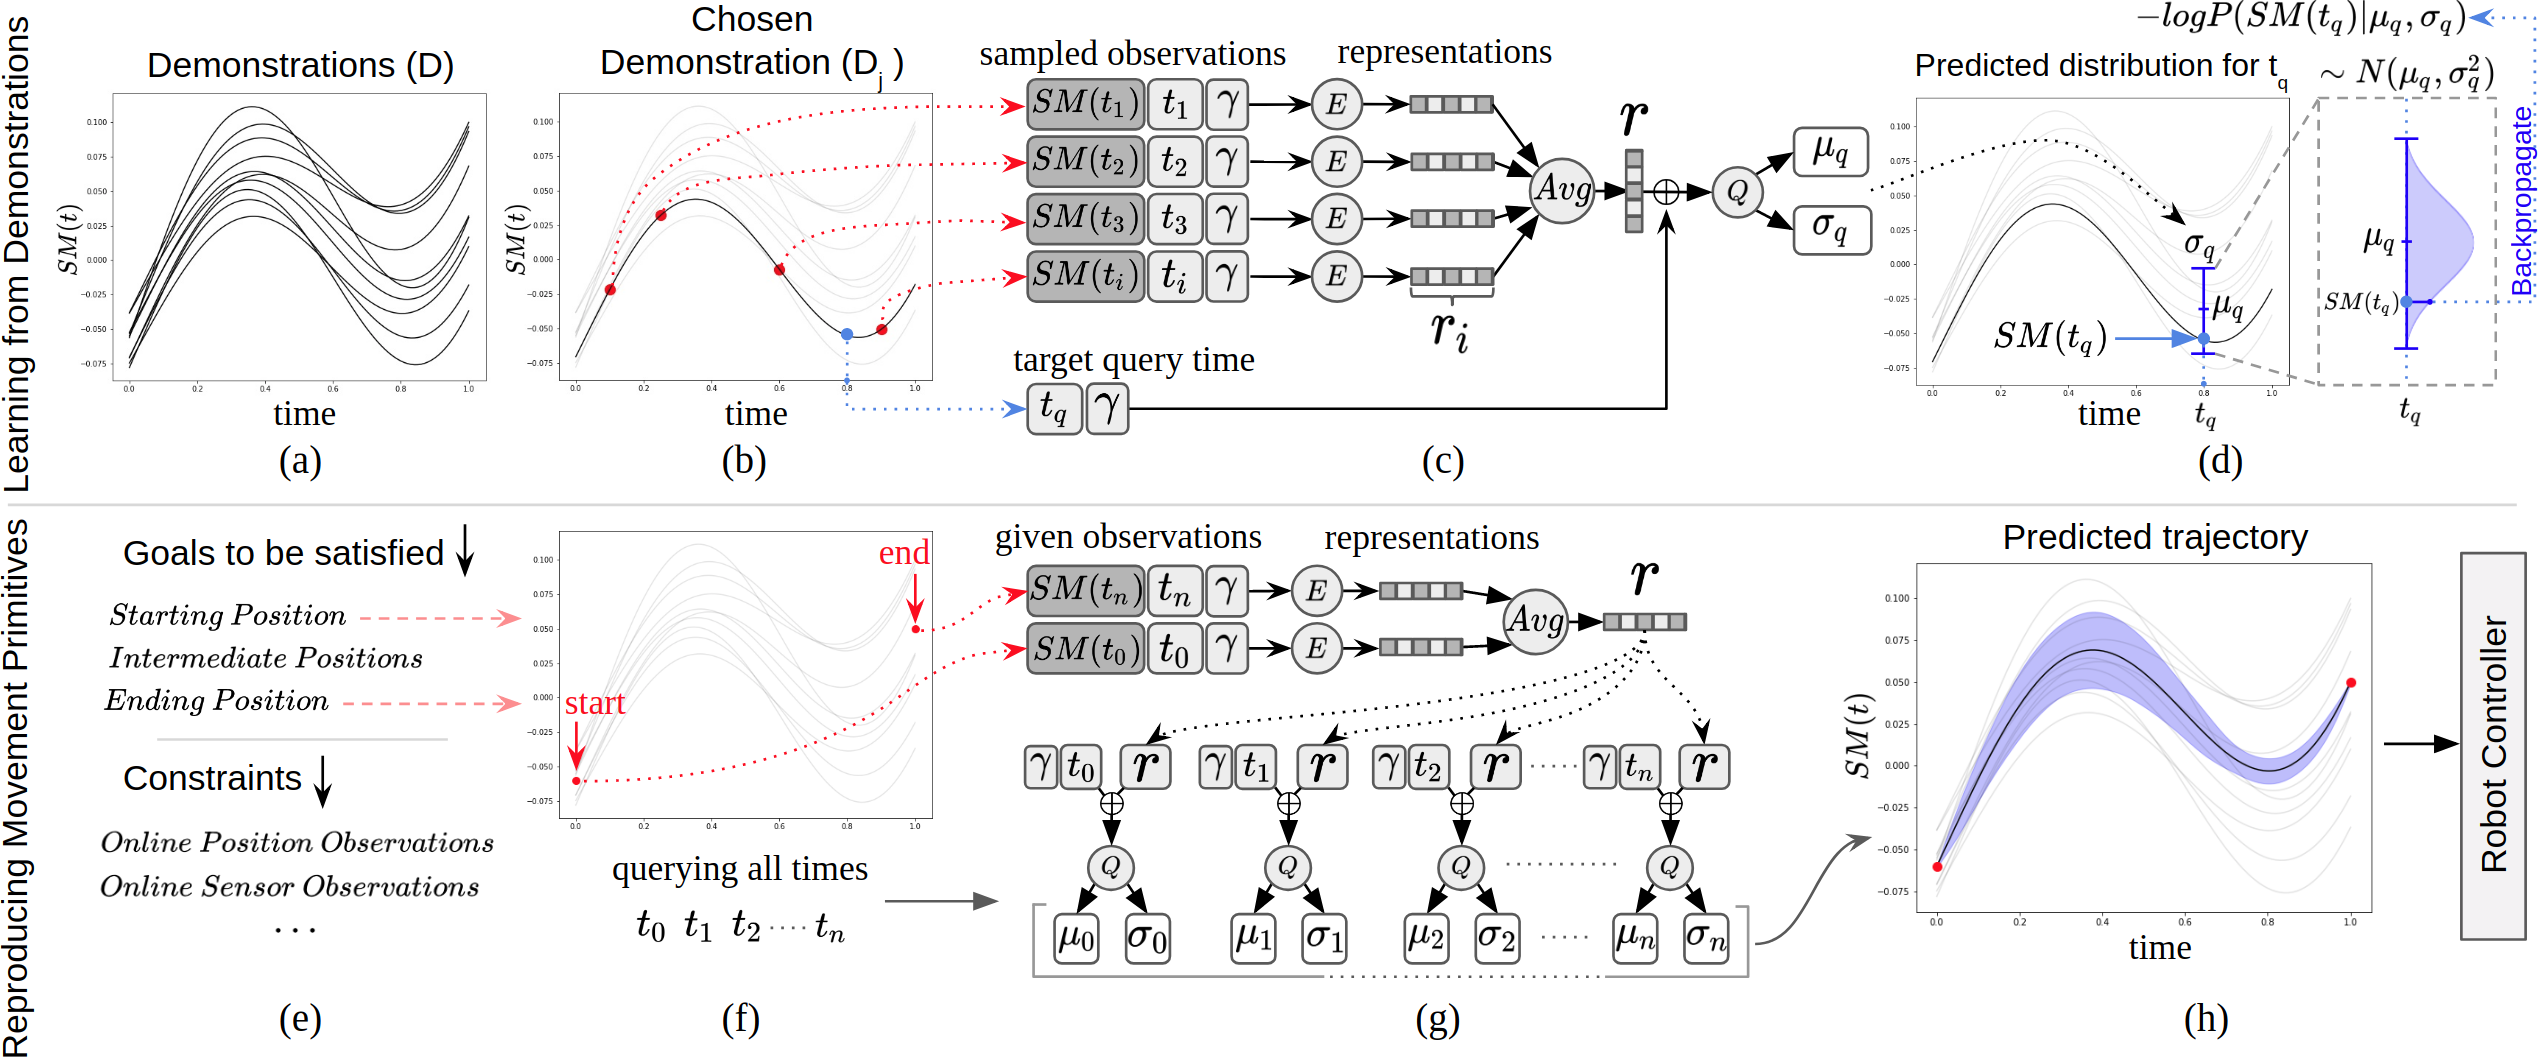
\includegraphics[width=0.9\linewidth]{Images/CNMP.png}
	\caption{CNMP model, it is conceived to work with temporal relations between sensorimotor data and different task parameters}
	\label{fig:cnmp}
\end{figure}
The "learning from demonstration" framework can learn non-linear relationships between trajectories and reproduce them in joint or task space. In this case, a trajectory is formally defined as a temporal function, $\tau = \tau (t)$, where the sensorimotor data in time describes how a robot moves. So, each trajectory $\tau$ is a list of ordered sensorimotor values: 
\begin{equation}
    \tau = \{ SM(t_1), SM(t_2), ... , SM(t_T ) \}
\end{equation}
where $SM(t_i)$ is the sensorimotor data at an instant of time $t_i$.
So, the challenge of trajectory generation becomes figuring out a series of commands $SM(t_i)$ that creates the movement desired \cite{gasparetto2007new}. 
Finally, with a set of observations $O$, the model has to learn the function $\tau = f(t|O)$, using $N$ expert demonstrations, $D = \{\tau_1, \tau_2, ... , \tau_N \}$. 

CNMPs are conceived to work with temporal relations $t$ and different task parameters $\gamma$. CNMPs maintain the permutation invariance of CNPs over observations $O$ and queries $T$. Furthermore, to make the model time-invariant, the sensorimotor trajectories are often scaled in the interval [0,1]. 
The task parameter $\gamma$ effectively adds one or more dimensionalities to the network's input, and it's passed to both the encoder and the decoder. An observation becomes the concatenation of $SM(t_i)$, $t_i$, and $\gamma$. The dimensionality of $SM(t_i)$ depends on factors like the Degrees of Freedom of the robot joints and the number of variables corresponding to the actuators. 
For the aggregation of the representations, the averaging operation has been chosen.
During training, a random trajectory $\tau_i$ is selected from the $D$ set of expert demonstrations. Next, a random number $n$ of random observation points are selected from the trajectory $\tau_i$. The encoder takes the $n$ observations and produces $n$ representations. The final representation is obtained by averaging the representations produced by the encoder fed with all the observation points. 
The target data is predicted using the representation and the query time $t$ concatenated to the task parameter $\gamma$

The encoder and the decoder are trained jointly with the error calculated from the following loss function:
\begin{equation}
    L(\theta, \delta)= -logP(y_i|\mu_i, softmax(\sigma_j))
\end{equation}
using both mean and standard deviation produced by the network.
As a note, the uncertainty of the prediction provided by the variance is useful for the model's active exploration to choose wisely where the next observations are needed.
Moreover, the capacity of CNMPs to deal with high-dimensionality input can also be used to input images in the model. Image completion indeed can be seen as a regression task.
Leveraging the interpolation capabilities of CNMPs, our approach will investigate novel synthesis by combining and concatenating previously taught ones.
    %----------------------------------------------------------------------------------------
\chapter{Platforms}
\label{chap:platforms}
%----------------------------------------------------------------------------------------
In this chapter, all the physical and digital platforms utilized will be explained to give a proper understanding of the initial architecture and a more comprehensive idea of the environment of the experiments. The first part will state the devices and their setup, capabilities, and configuration used. Subsequently, the frameworks and libraries employed will be listed and described. 

\section{Baxter Robot}
The Baxter robot is an industrial robot built by Rethink Robotics in 2011 \cite{wiki:baxter}. The platform [Fig. \ref{fig:baxter}] has two robotic arms with interchangeable grippers at the wrist (End Effectors). The robot is 180cm tall and, with its pedestal, weighs 140 kg. The arms have 7 degrees of freedom (DOF), which implies they have seven joints each. This makes it kinematic redundant, meaning that for some points reached in space, multiple pose configurations of the arms are possible. These two factors combined allow the robot to have an impressive capability in manipulation. The robot can be equipped with suction caps or two-jaw parallel grippers; we chose the last ones in our configuration. The gripper, in addition to its position, also offers information regarding the force applied while grasping an object.

The robot was designed with attention to collaborative tasks with humans. For this reason, it eases teaching by demonstration by having integrated two touch sensors in the wrists that unlock the motors of the arms, allowing the user to move them easily and record the trajectories executed. The robot helps the movement with a feature called "Zero-g mode", in which the weight of the joints is neutralized actively by the motors. This enables the teaching expert to demonstrate movements in a similar environment without gravity, without having to carry the instrumentation load in time constantly. Furthermore, the robot has many input buttons and LEDs, they are present on the hands, arms, and chest, and they allow the programming of custom behaviors. They are especially useful in retrieving and giving instructions to the robot without reaching a computer, like closing the gripper at the desired moment, getting feedback, or starting the trajectory recordings. 

Another feature worth mentioning is the increased safety of operating around humans. Thanks to active and passive safety systems equipped in the platform, it doesn't require a cage for protection. On the other hand, making the robot less hazardous comes with the cost of precision. A motor driving a spring that drives Baxter's arm instead of just a direct motor impacts the precision of movements, sometimes in terms of centimeters. This doesn't make the robot perfectly suitable for industrial applications, but especially appropriate for research and for the adaptability in our project.

The head of the robot includes a ring of sonar sensors for people detection, a wide-angle camera, and a movable display that acts like a face. 
Another benefit of the robot lies at the end of both hands. Immediately next to the attachment for the tools, an infrared (IR) sensor provides data on the distance from a solid object (i.e., a table) and an inertial measurement unit (IMU). Moreover, an embedded RGB camera is also present, allowing to see closely the object approached or to change the point of view on it without additional external cameras.

\begin{figure}
	\centering
	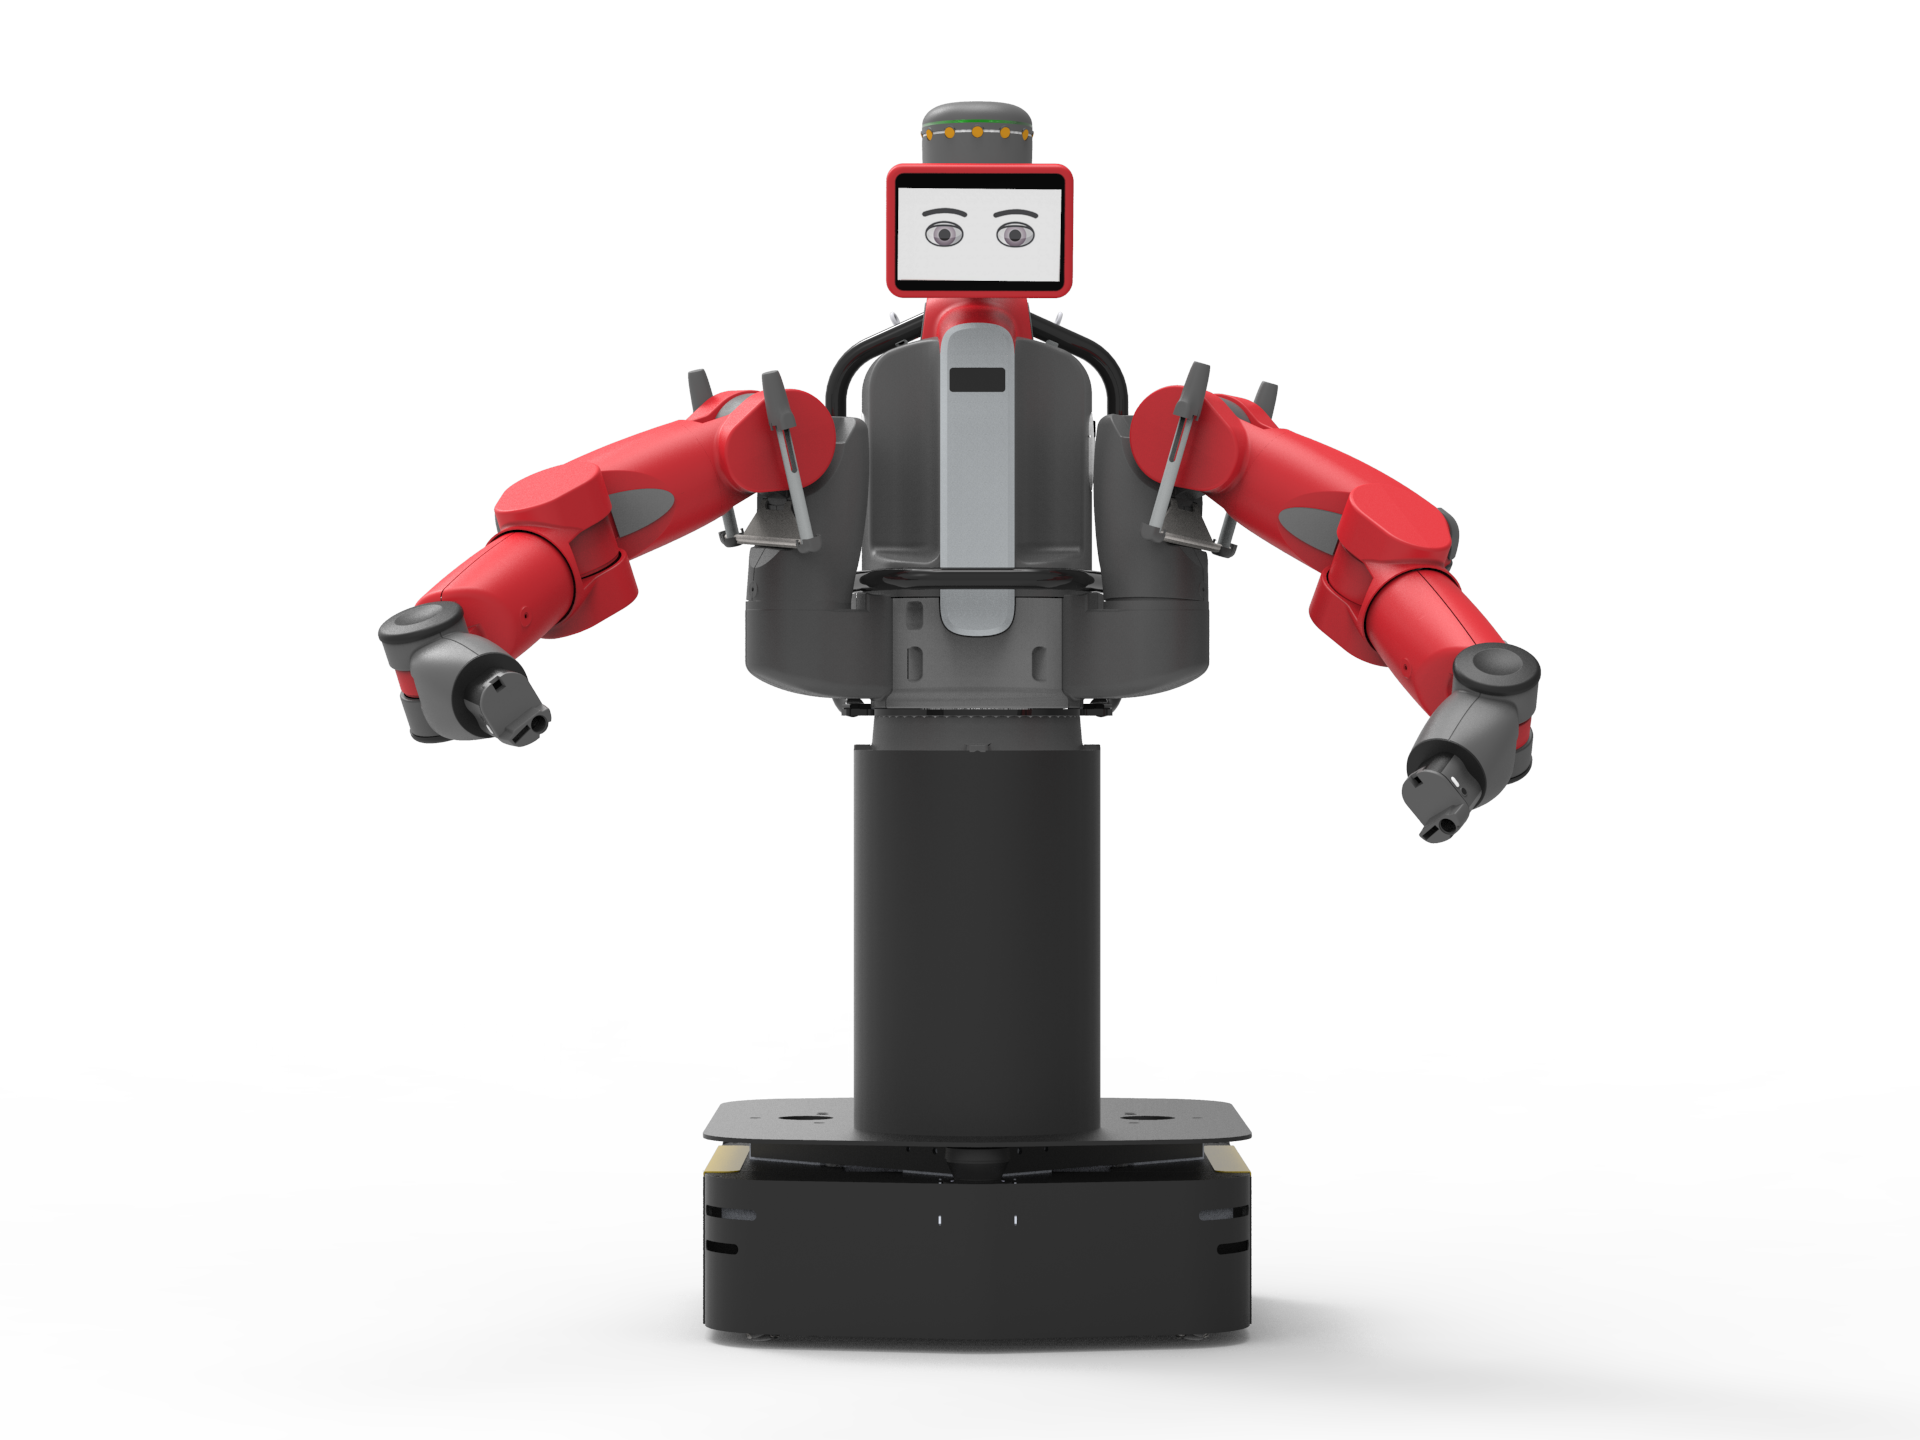
\includegraphics[width=0.5\linewidth]{Images/baxter.png}
	\caption{Baxter Robot platform}
	\label{fig:baxter}
\end{figure}

\section{UR10 Robot}
UR10 is a single industrial robot arm that shines in reliability and precision [Fig. \ref{fig:ur10}]. It has been manufactured by Universal Robots and combines long reach with a high payload \cite{url:ur10}. It is intended for medium-duty tasks, so it's compact in its overall dimensions compared to a fully intended industrial robot. It can reach an impressive height of 2.3m on its pedestal. In our experiments, it was mounted on a pedestal 0.85m tall to increase the reachability at table level. 

The arm has a reaching radius of 1,3m from the mounting point, which implies a workspace of approximately 5,3 square meters at the base level. The robot has 6 Degrees of Freedom, with six rotating joints. It is able to reach any point in its reaching radius but has no kinematics redundancy, meaning only one position is possible for any given point. The total payload that can be carried is 10 kg. 

\begin{figure}
	\centering
	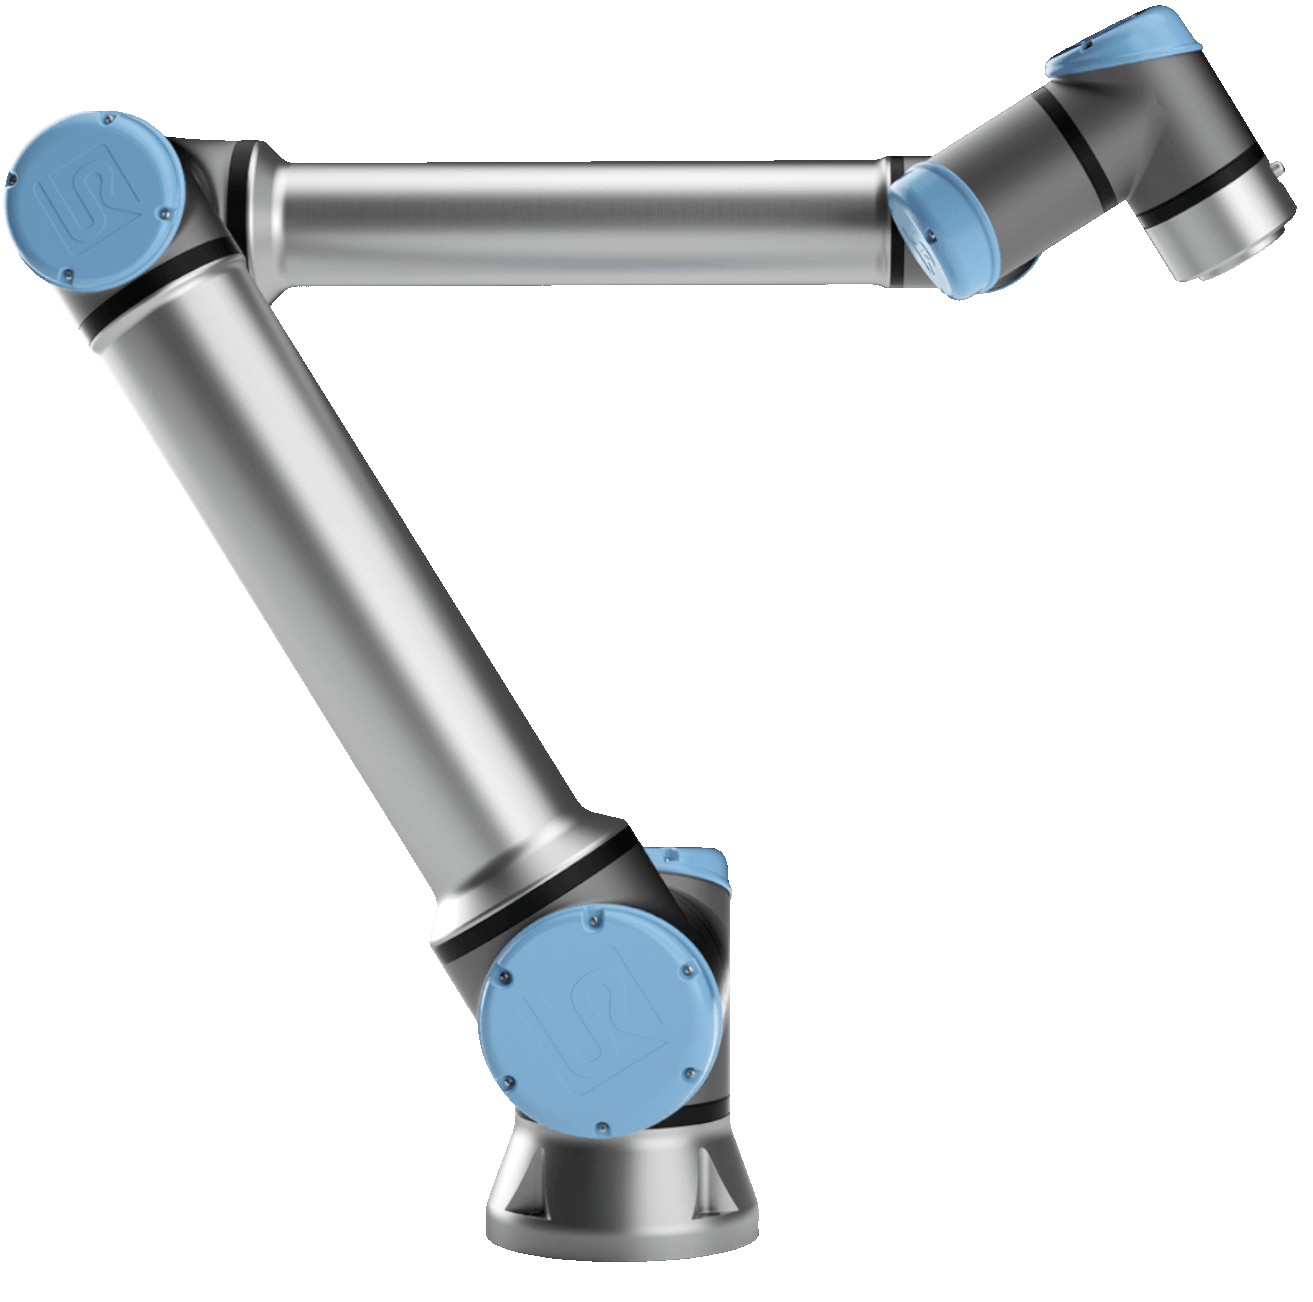
\includegraphics[width=0.5\linewidth]{Images/ur10.png}
	\caption{UR10 Robot platform}
	\label{fig:ur10}
\end{figure}

Like the previous robot, this one is designed to work collaboratively with humans. It features built-in safety features, such as force/torque sensors, to detect and respond to external forces or unexpected events. A button to release the motor breaks is present on the floating touch screen and allows the robot's motion by hand. This robot also doesn't require a safety cage around for protection, but the emergency stop button always has to be within easy reach. 

The robot design emphasizes modularity, making it easier for users to customize and adapt it for different tasks or use various end effectors. We coupled it with a three-finger gripper described in the next paragraph.


\section{3F Robotiq Gripper}
At the end of the UR10 Robotic Arm, a Robotiq 3-Finger Adaptive Robot Gripper was mounted [Fig. \ref{fig:gripper3f}]. The gripper has a human-inspired design and has three fingers with three joints each \cite{url:3fgripper}. The physical platform was chosen for its precision and safety, and it pairs well with the UR10 capabilities. The gripper offers different grip modes; the ones available are: "basic", "wide", "scissor" and "pinch". Each is appropriate for distinctive objects to grip; the basic one is the most versatile, but the wide one has more stability for big or long objects, and the pinch one is the best for small objects. The "scissor mode" closes together the two fingers on the same side, for high-precision manipulation. We mainly used the "pinch" setting. 

\begin{figure}
	\centering
	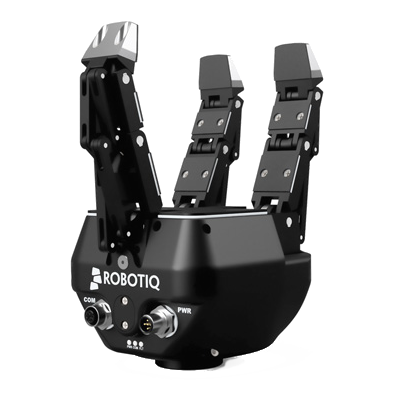
\includegraphics[width=0.5\linewidth]{Images/gripper3f.png}
	\caption{3F Robotiq Gripper platform}
	\label{fig:gripper3f}
\end{figure}

The gripper has a mass of 2.3 kg in contrast with a grip payload of 10 kg. The grip force applied can range from 30 to 70 N, depending on the grip mode selected. The precision declared is up to 0.05 mm.

This platform was designed as well for collaborative robotic applications, allowing it to work safely alongside human operators. It incorporates safety features to detect and respond to external forces, stopping in case of high forces applied. The torque and speed of gripping data are available and exposed through a dedicated ROS topic. Speed and torque are also adjustable for the intended use. It is possible to control and retrieve data for each finger individually. 



\section{FT 300-S Force Torque Sensor}
Between the UR10 robot and the 3F Finger Gripper, an FT 300-S Force Torque Sensor [Fig. \ref{fig:ft-sensor}] was mounted to increase precision and repeatability. The sensor offers high-resolution real-time measurements regarding the force and torque applied to the three space dimensions and improves the capabilities of the robot, making it able to detect the payload carried or the amount of pressure between the object carried and the static environment (i.e., the table). 

The device was built for compatibility with the Universal Robot series and has an IP65 rating. It also enables precise object placement such as alignment, indexing, and insertion \cite{url:ftsensor}. The FT 300-S is commonly used in tasks where force and torque sensing are critical, but we used it to increase the reliability of the payload measurements. 

\begin{figure}
	\centering
	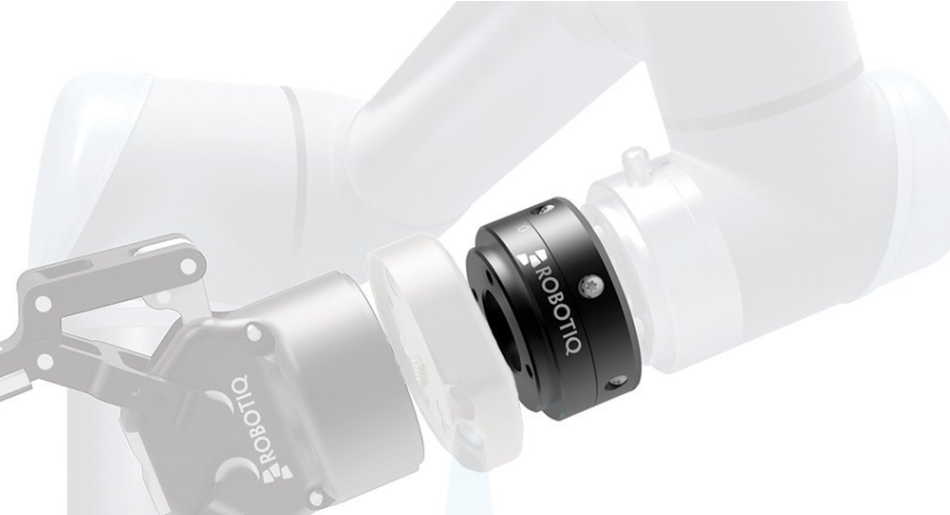
\includegraphics[width=0.5\linewidth]{Images/ft_sensor.png}
	\caption{FT 300-S Force Torque Sensor}
	\label{fig:ft-sensor}
\end{figure}


\section{Frameworks}
\paragraph{ROS}
The Robot Operating System (ROS) \cite{url:ros} is a framework to standardize the deployment of robot applications. The system is a set of software libraries and tools that combine the state-of-the-art drivers for the most common robot interfaces and contain the most used algorithms for robotics. 

Since robotics programming is a complex challenge, the idea behind ROS is to use the "divide et impera" approach and split it into multiple sub-problems. This division requires a distributed strategy, and distribution implies communication among parts. One of ROS's main objectives is to standardize communication. For this reason, ROS acts like a middleware framework, allowing the ease of the dialog between software and the robotic hardware. It is widely used in research and industry, from mobile robots to manipulators. In our research, we used ROS version 1. 

It's platform-independent and open source, so it is possible to create a custom robotics device compatible with it, and it's possible to develop personalized libraries. Its modular architecture allows the creation or use of a series of executable pieces of code called nodes, which run on a single or even on many computers. The nodes communicate among themselves with messages in the form of data structures previously defined. The distributed system allows to decuple the computation of heavy tasks, like vision, 3D reconstruction, and navigation, from the robot's hardware. 

Communication occurs through "topics" and "services". Nodes running on any computer ping the "master node" designated to retrieve all the possible topics and services exposed from other nodes in the network. A node can be a "publisher" or "subscriber" to a topic, sending messages to it or receiving messages from it. Communication with topics is not blocking and it is many-to-many: multiple nodes can publish, and simultaneously, multiple nodes can subscribe to a topic. Services work in a similar way, but the communication blocks the computation till the data requested is retrieved. Their mechanism is analogous to Remote Procedure Calls (RPCs). 

ROS is available with two commonly used programming languages: Python and C++. We used the Python version with the "rospy" package in the experiments with both robots.

\paragraph{Pytorch}
Pytorch is a Deep Learning framework \cite{paszke2019pytorch} that focuses on speed and usability with an imperative and Pythonic programming style.  The Python library \cite{url:pytorch} offers a wide variety of models and building blocks for constructing neural networks. By design, it eases the debugging for the user with a rich ecosystem of dedicated tools. It works on the CPU and on hardware accelerators like GPUs. For this reason, PyTorch provides a multi-dimensional array called a tensor, which is similar to NumPy arrays. Conversions among both of them will be present in the code implementation. 

\paragraph{Jupyter Notebook}
Jupyter Notebook is an open-source interactive web application \cite{url:jupyter}. It supports multiple programming languages and offers a cell-based environment where code and description/graphical results can be blended. Jupyter Notebook integrates seamlessly with popular Python libraries, such as NumPy, Pandas, Matplotlib, and scikit-learn; some of them will be described later. It was used occasionally in our experiments to provide a fast and interactive coding experience with Python. The notebooks can be easily shared, and the process is clearly visualized. It was specifically useful in plotting multiple graphs during the training stages of neural networks or debugging operations on multi-dimensional arrays. 

\paragraph{Anaconda and Python Libraries}
Anaconda is an open-source software that contains open-source tools and packages for data science, machine learning, and scientific computing \cite{url:anaconda}. It has been used to track the packages utilized in the robotic platforms and in the models' development and training. The Conda package manager was the most used tool to easily install, update, and manage various software packages and dependencies. Some of the most important libraries are listed below.
\subparagraph{MatplotLib} Matplotlib is a comprehensive 2D plotting library for Python that generates high-quality charts, plots, and visualizations. It has been widely used to double-check the quality of the training or plot the trajectories recorded with the robots. 
\subparagraph{Numpy} NumPy is a package for numerical computing in Python. It supports large, multi-dimensional arrays and matrices and a collection of mathematical functions to operate on these arrays. It has been used for array slicing, normalization, and smoothing data. 
    %----------------------------------------------------------------------------------------
\chapter{Design} 
\label{chap:design}
%----------------------------------------------------------------------------------------

In the previous chapters, it has been presented the necessary knowledge about the background research (\cref{chap:background}) and the platforms utilized in this work (\cref{chap:platforms}). 
This chapter discusses the conducted research from the design perspective, giving the main points and emphasizing the key ideas without going into the implementation details as the next chapter (\cref{chap:implementation}). 

As analyzed in the Intro (\cref{chap:introduction}), humans have remarkable cognitive flexibility and use it to achieve complex goals across various daily scenarios. These goals are often broken down into smaller sub-tasks (skills), and this is one objective of this research. This combination of trajectories also requires an appropriate shift among them, in both cases, the combination being end-to-end or partial. 

Being biologically inspired, this research aims to emulate this human flexibility in skill execution and task composition with the previously explained CNMP networks. Movement primitives that define skills are combined differently for different goals and are adapted to the environment and context thanks to the interpolation abilities of CNMP networks.

The following discussion will proceed with analyzing before the partial skill composition with CNMPs, modeling how it is possible to go from one movement primitive to the other. The motivation of this order is that this part enables the partial combination and is used as well in the transition moment of end-to-end skill concatenation. 
Next, it will be analyzed how it is possible to concatenate them one after the other to achieve meaningful execution in order to reach the final goal position or even goal-state.

\newpage
%%%%%%%%%%%%%%%%%%%%%%%%%%%%%%%%%%%%%%%%%%%%%%%%
\section{Partial Skill Combination}
%%%%%%%%%%%%%%%%%%%%%%%%%%%%%%%%%%%%%%%%%%%%%%%%

% requires change action (shift TP) halfway
In order to synthesize a new skill by combining parts of others, it is required to teach the model at least two different types of movement primitives. Subsequently, the robot has to be able to pass from one action (skill) to the other. The moment of this transition has to be arbitrarily decided according to the necessities and not specifically crafted at teaching time. 

The challenge of this apparently straightforward problem resides in the moment of the transition, because it has to be executed in a meaningful, natural, and safe way. These simple three requirements will lead the following examination through different approaches till the one designed. 

For the purpose of a better understanding of the design and its steps, from now on, a simplistic example (\cref{fig:trajX}) will be used to further clarify the explanations given. Nevertheless, the simplification doesn't exclude the possibility of more elaborate tasks that require complex movements or sensorimotor data. The two actions discussed will be a simple movement upwards and a similar movement downwards. They can represent, for example, a trajectory in real life, a manipulator movement, or a joint trajectory. This allows a discussion that starts from a single 1D dimension and keeps the understanding manageable at the subsequent introduction of new dimensions. 

\begin{figure}
    \centering
    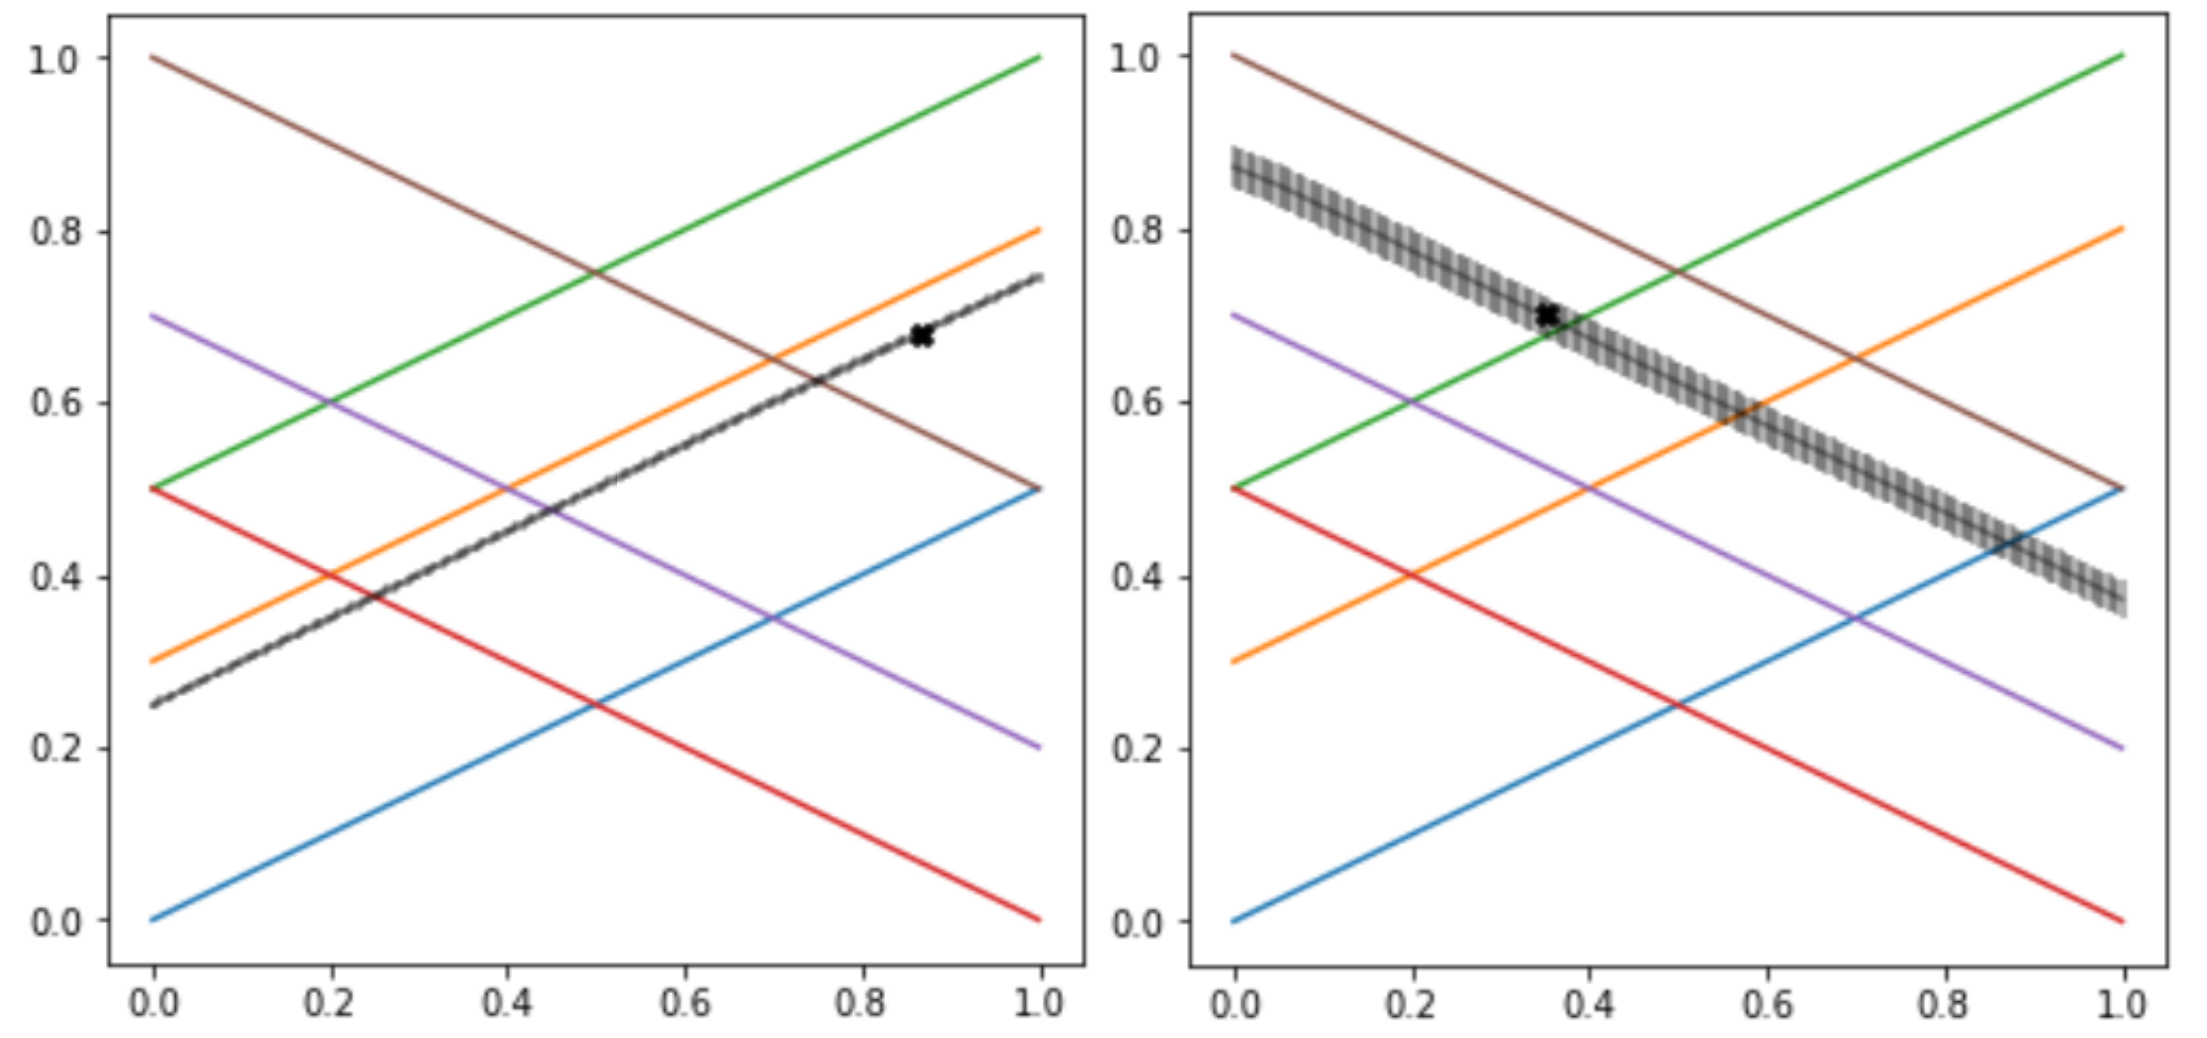
\includegraphics[width=0.8\linewidth]{figures/trajX.png}
    \caption{Trajectories for two different skills demonstrated and generated ones from the conditioning points.}
    \label{fig:trajX}
\end{figure}

Some demonstration trajectories are given for both skills, in the \cref{fig:trajX} are visible as the three colorful thinner lines ascending and three colorful thinner lines descending. The two triplets differ to some extent, so the network has enough knowledge to create as well new trajectories never seen. This will prove later that the method designed also works with newly generated movement primitives. 
The thicker points in the \cref{fig:trajX} are the conditions, these force the model to generate a trajectory that passes through that state. The movement primitive created is denoted as the grey line passing through the condition point, along with the uncertainty of the prediction in every timestep as its width. 

% do it without jumps
The shift can not be abrupt, so it's not sufficient to directly stitch together two parts of the trajectories collected. 
The simplest solution of executing one trajectory till a certain desired timestep and executing the second one after that moment will create an abrupt jump in the execution for the majority of timesteps where the trajectories don't perfectly intersect (\cref{fig:trajX-failing-approaches}). A jump in the movement primitive will lead to an unnatural fast change of pace and position of the robot during the execution, which not clearly referable to human behavior. Moreover, moving from one position to a completely different one in the next moment is an unsafe behavior. It might lead to damage to the robot itself and its surroundings, harm to people, or activate the safety stop measures of the robot due to the high speed and torque applied.  

\begin{figure}
    \centering
    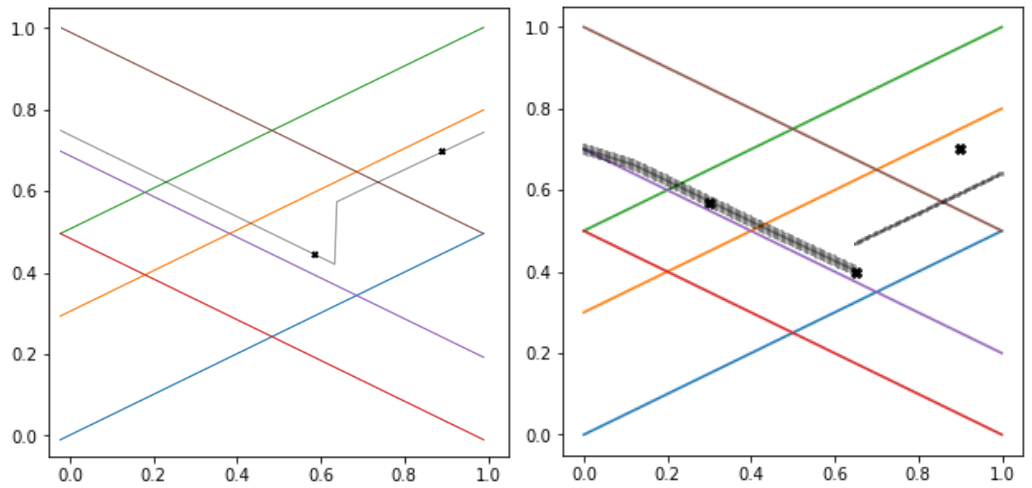
\includegraphics[width=0.8\linewidth]{figures/trajX-failing-approaches.png}
    \caption{Examples of failing approaches with stitching in CNMPs. On the left, simple combination of parts. On the right, stitching the right part using a conditioning point at the end of the left part.}
    \label{fig:trajX-failing-approaches}
\end{figure}

Being able through the CNMP model to generate trajectories from previous demonstrations allows a certain flexibility, so a second approach might suggest generating a second trajectory starting from the end points of the first one. This solution only delays the problem subsequently because the condition point(s) on the second trajectory will be dependent on the first one, and this requires further calculation, and won't be solely used for the effective purpose of making a trajectory reach the desired state. In \cref{fig:trajX-failing-approaches}, right plot, the first part of the trajectory is generated with the left-most condition (time 0,3). Subsequently, the second part is generated using a conditioning point at the end of the left part plus the desired one. These two conditioning points will likely not be on the same trajectory generated: let's recall the robot arms generally have 6 or 7 DoF, \cref{chap:platforms}, and even the cartesian space has three dimensions plus the 4D quaternion for the orientation, so the probability of trajectories intersecting in spaces of at least six dimensions is minimal. This will lead the CNMP model to average the two trajectories obtained by the two conditions on different points. In \cref{fig:trajX-failing-approaches}, right plot, we see the second trajectory part passing in the middle of the two right-most observations that would generate independently two different movement primitives. To pass from one to another of these last two trajectories, a shift will still be required, and this raises again the same problem. 
So, even using conditioning points, there is a tradeoff between jumping and not meeting the conditions for the second trajectory.

% same network
Since the stitching of parts is not a feasible option, the approach selected implies giving the same network the two skills and obtaining a coherent output.
% uncertainty of some observations
The CNMP model is capable of storing different movement primitives of different skills without requiring multiple networks. The selection of the right trajectory is due to the conditioning points (observations) previously explained. The observations are indeed useful for both finding the interpolated trajectory from the demonstrations passing in a new state and also for identifying the correct skill. In \cref{fig:trajX}, the conditioning points identified uniquely the trajectory to generate. However, as it happens in \cref{fig:trajX+tp}, the conditions might be uncertain, so the standard CNMP model averages the outputs, creating a misleading trajectory. 
% introduction TP to eliminate uncertainty
To eliminate uncertainty, a task parameter $\gamma$ (TP) can be included in both the input and the query of the network, as in \cref{fig:cnmp}. The task parameter is a full-fledged new dimension of the network, like input time $t$ and the output value. In the case of the task parameters, the dimension added is an input dimension, which excludes uncertainty. Now, the network, given a condition, can uniquely identify the movement primitive.
\begin{figure}
    \centering
    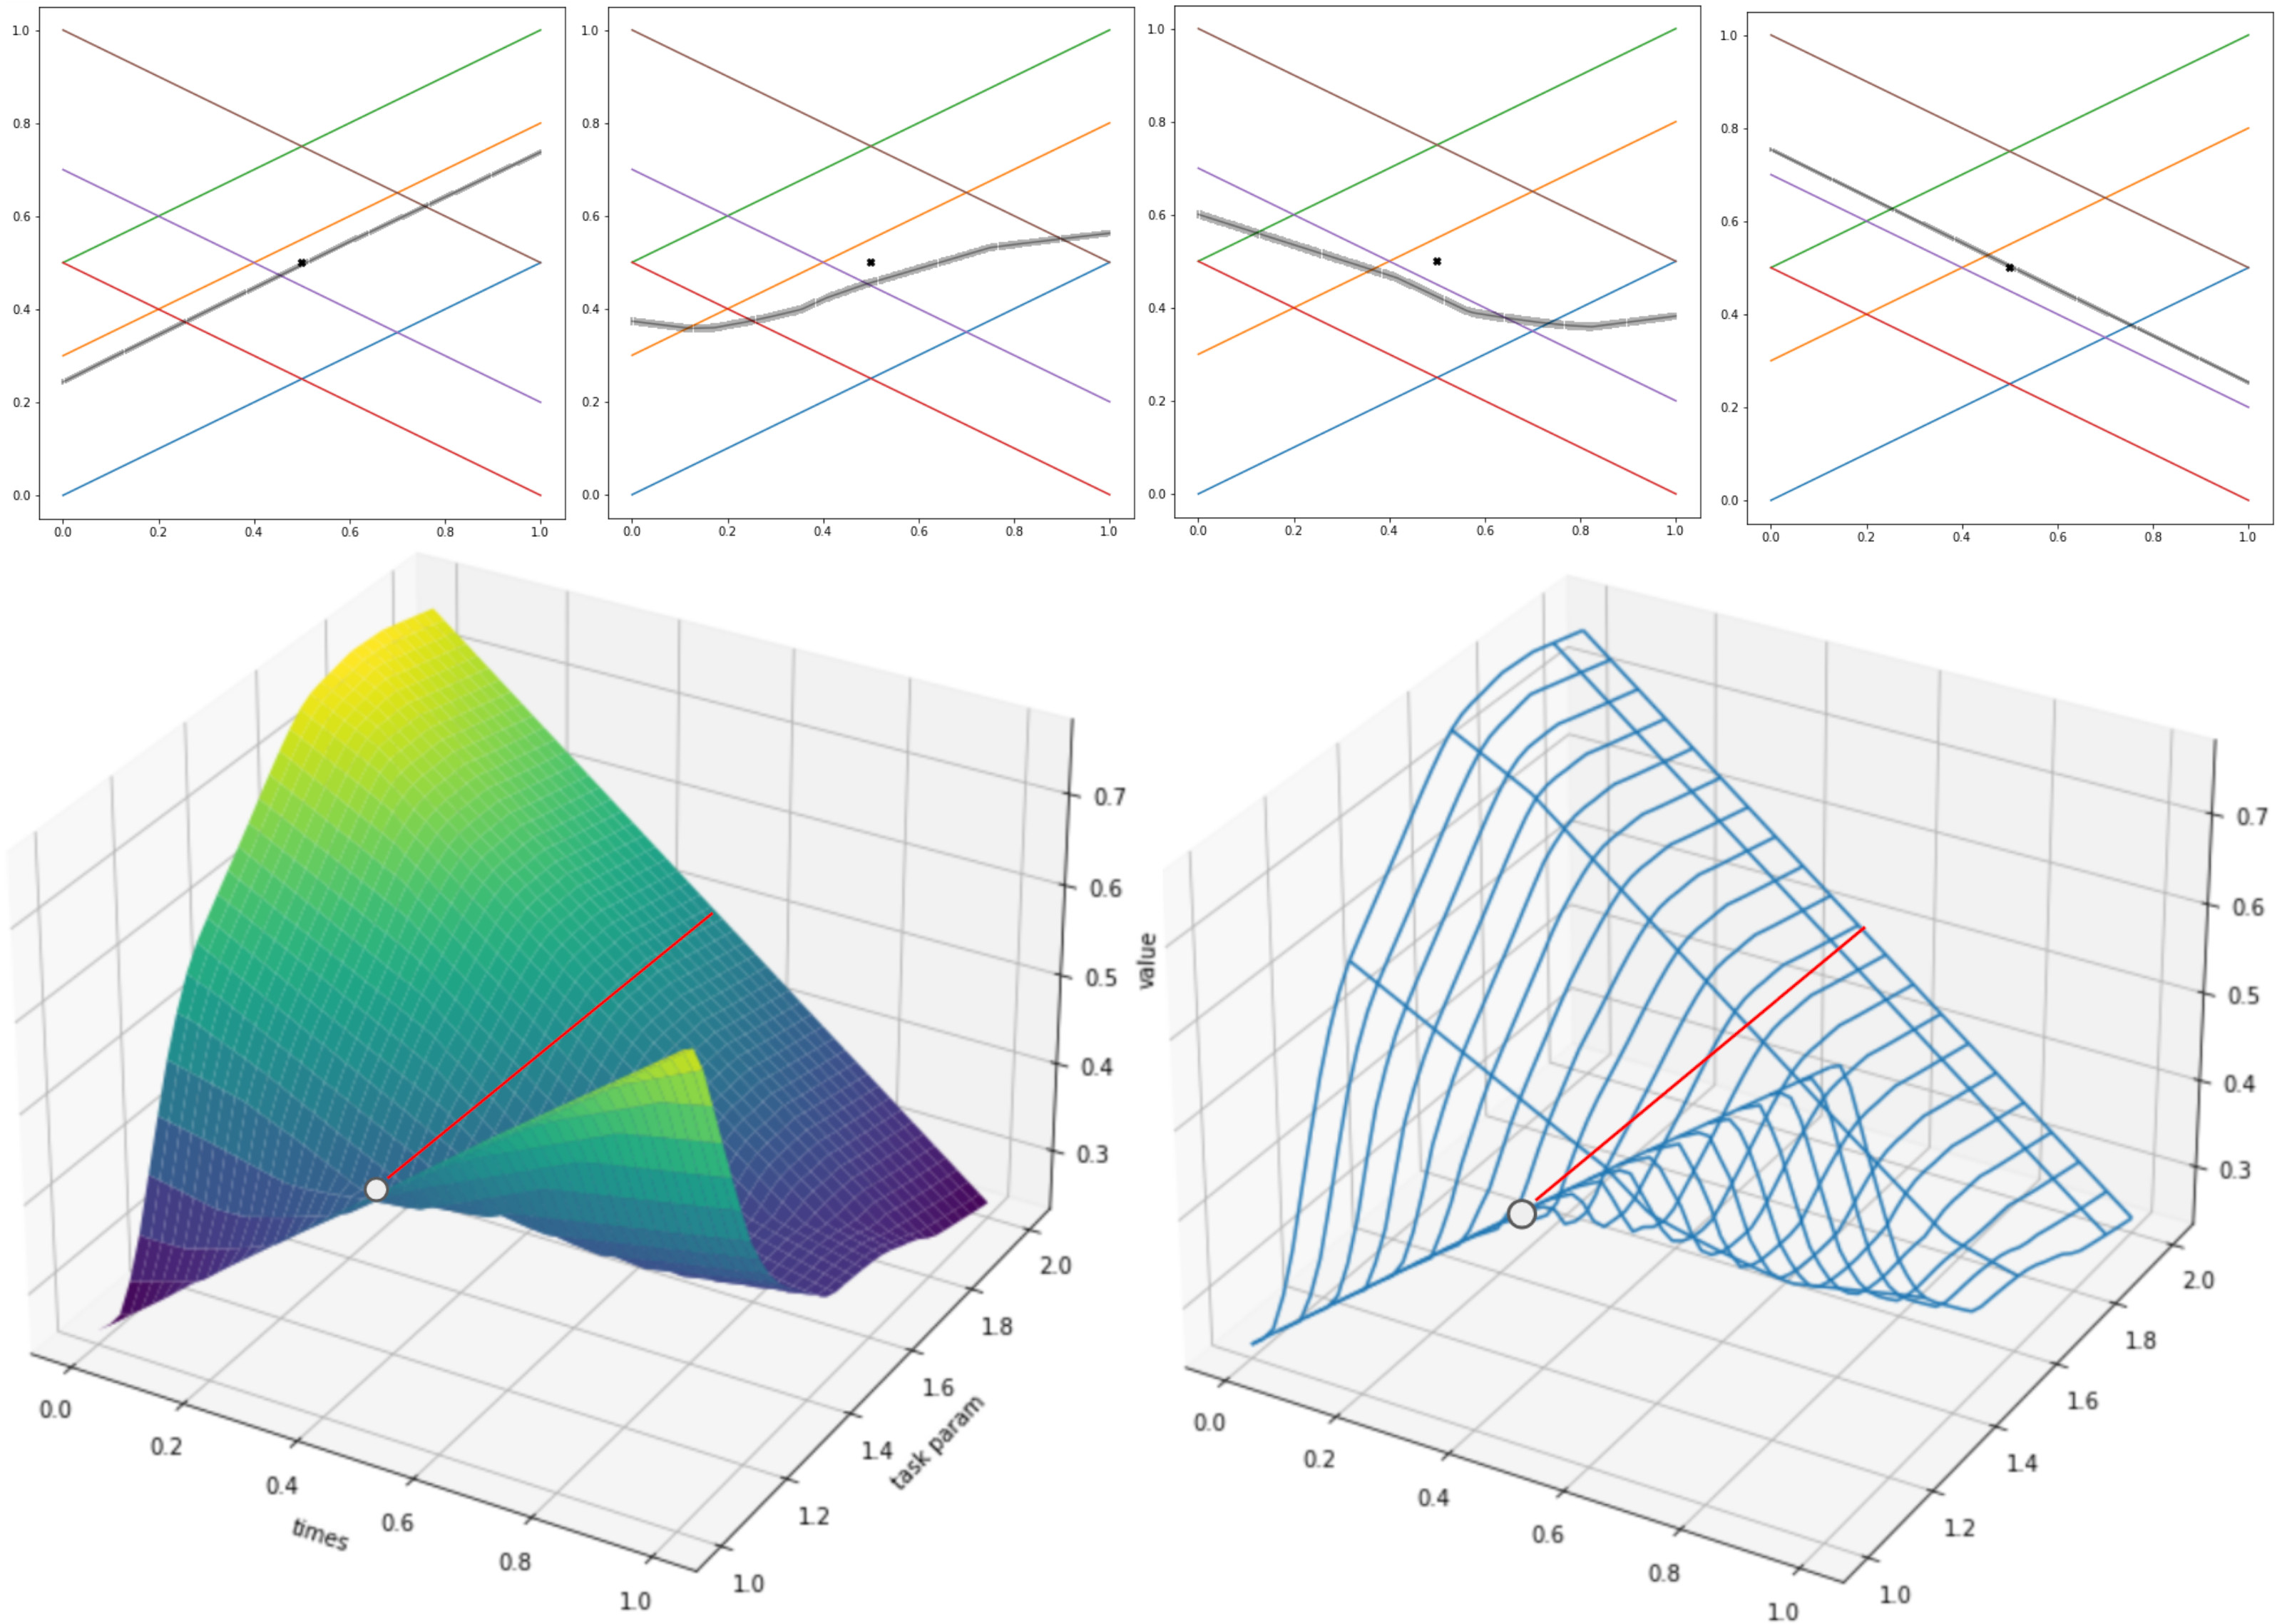
\includegraphics[width=0.9\linewidth]{figures/graph-tp-dimension.jpg}
    \caption{ Plot of the interpolation abilities of CNMPs also in the task-parameter dimension. }
    \label{fig:graph-tp-transition}
\end{figure}


\begin{figure}
    \centering
    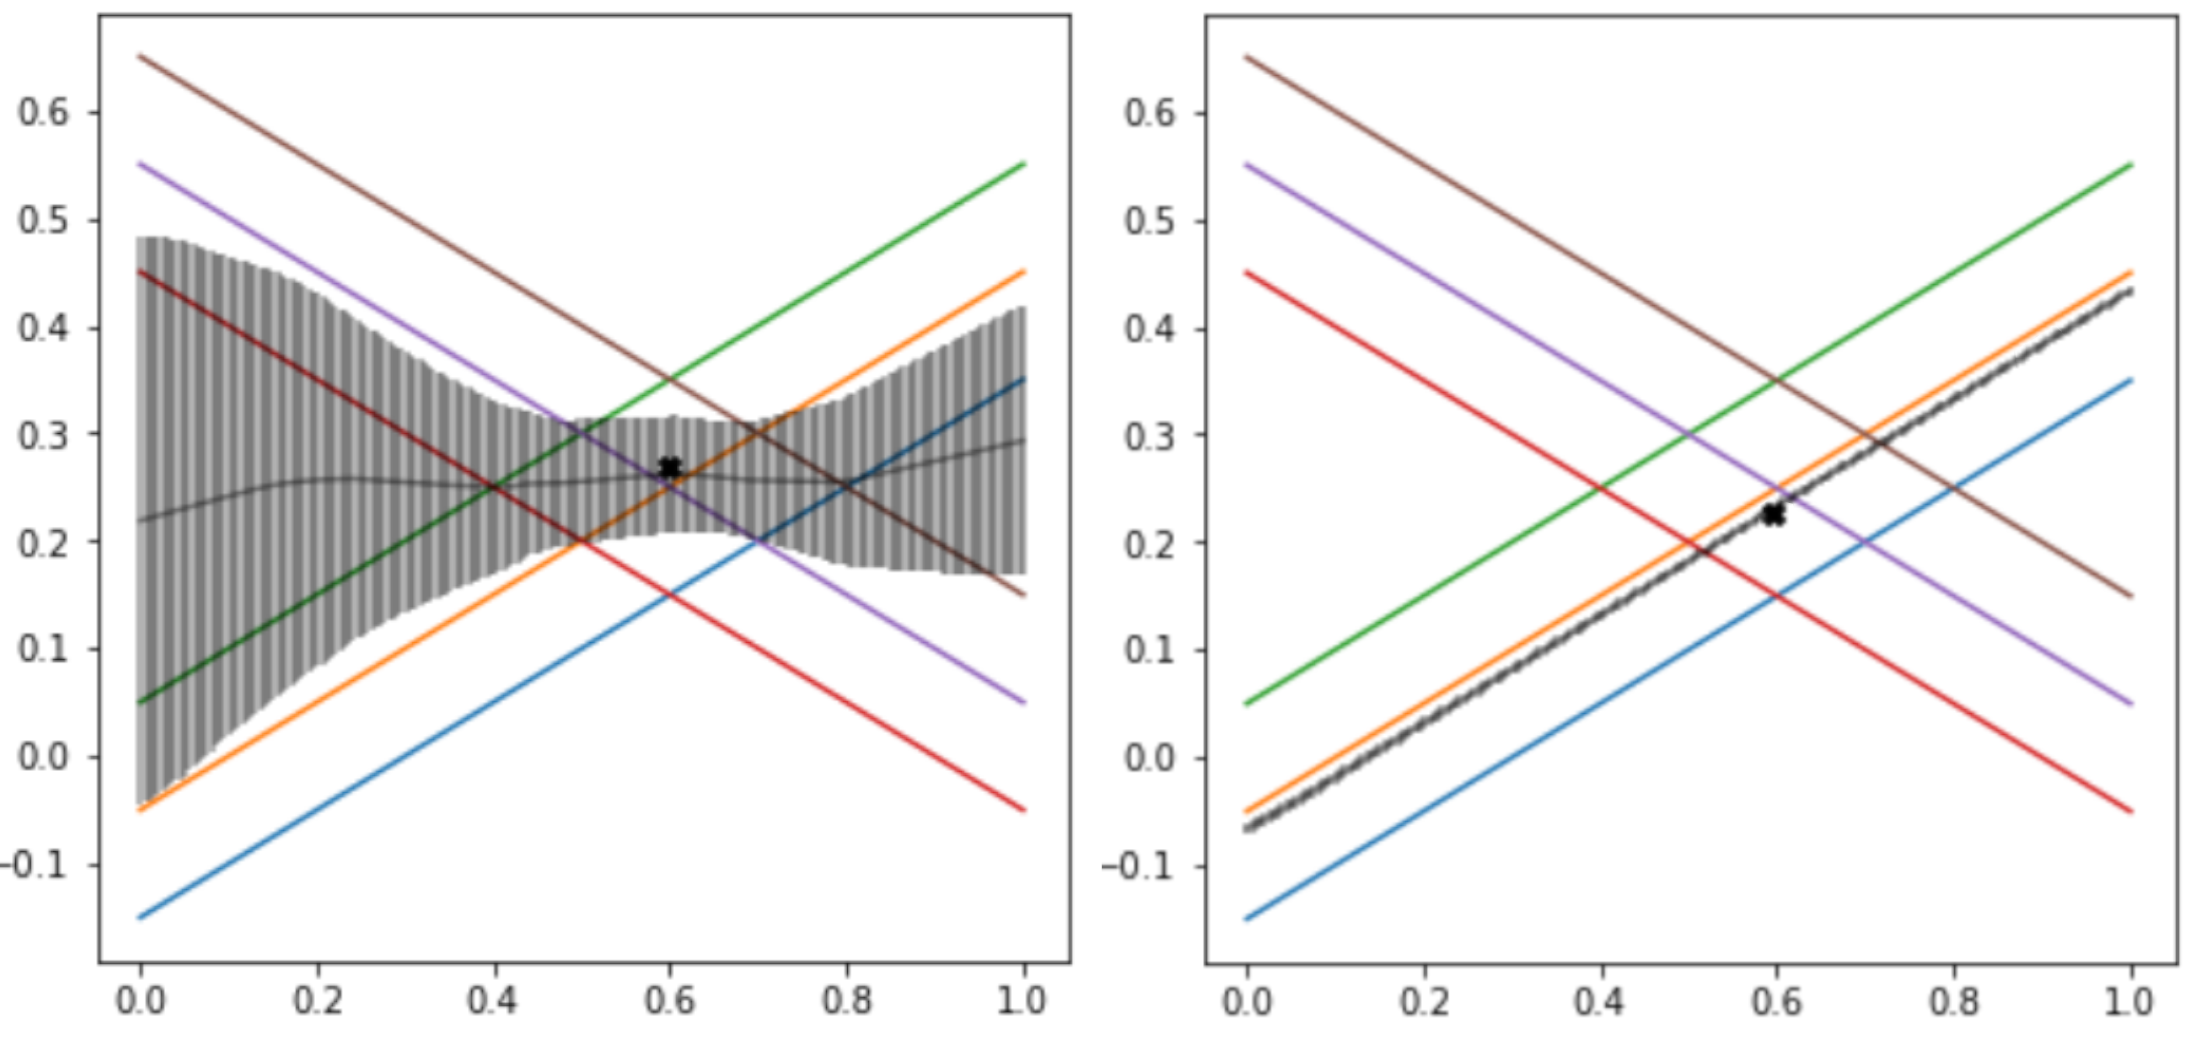
\includegraphics[width=0.8\linewidth]{figures/trajX+tp.png}
    \caption{ CNMP modeling uncertainty for a condition. In the parametrized CNMP, uncertainty is solved, and skills are encoded with task parameters 1 for ascending and 2 for descending. }
    \label{fig:trajX+tp}
\end{figure}
 
% What's among them? (using 1 condition) (shifting) network interpolates nicely
How adding a dimension to the input is interpreted by the networks and what's in between the two parameters has been researched to understand better how to shift among them. In order to do this, a 3D plot is required. This is achieved by leveraging the previously considered weakness of the model of having uncertain conditions. These points are shared by parameters among and maintain the same other dimensions while the external parameter $\gamma$ varies. This doesn't introduce any bias while the condition changes. The visualization of a continuous change between different task parameters is present in \cref{fig:graph-tp-transition}. As it's possible to observe, the network interpolates nicely among the functions also in the tasks-parameter space. The movement of the conditioning point in time is depicted in the 3D plot with a red line ending in its final position.
% network has 2 TP, in query and in observation, that varied together
It is worth noting that to obtain the graph in \cref{fig:graph-tp-transition}, both task parameters in the observations and in the query had to vary together. As visible in \cref{fig:cnmp}, the original network design of CNMPs implies the presence of this parameter (as $\gamma$) for the conditioning points and for the query $t$.

% if they don't? difference between observation and query, changing TP
Successively, the difference in variating only one at a time has been researched. In the first place, for all the time steps, only the task parameter of the condition was changed, maintaining the task parameter of the query constant. Next, the opposite was performed to understand how they influence the network result differently. The plots comparison is visible in \cref{fig:tp-influence}.
On the top row, for task parameter 2, the first graph shows how the result changes according to the variation of the task parameter in the condition. Meanwhile, the second graph shows how, for every time queried, keeping the parameter fixed to 2 in the conditions and changing it in the query doesn't produce a significant variation in the output. 
The second row repeats the procedure with the other task parameter to crosscheck the results. 
It is clearly emerging how the parameter in the observation seems to have a stronger influence than the one in the query, which doesn't seem to contribute significantly. 

The following subsections will investigate further the structure of the CNMP network and the design of two different architectures. This work proposes before a network with task parameters only in condition since it seems to be more influential, and next, the model with task parameters only in the query. These two architectures are respectively built and examined below.
\begin{figure}
    \centering
    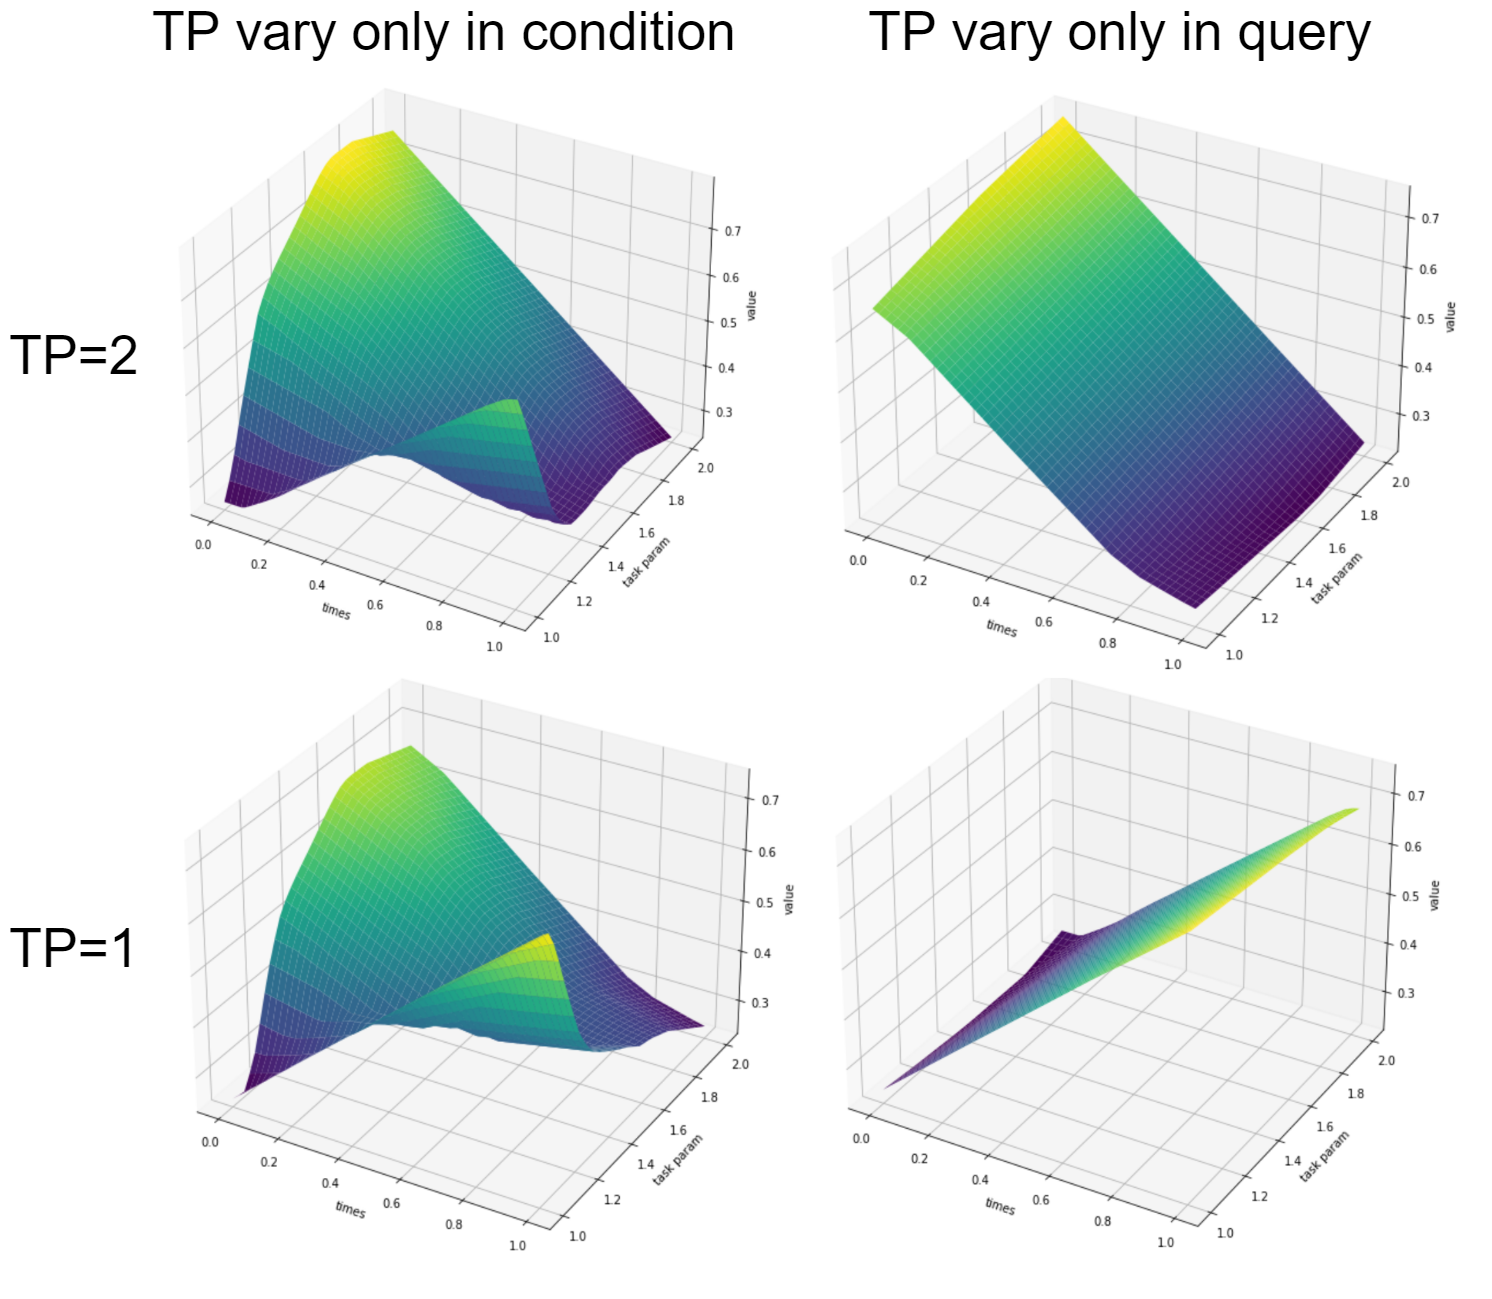
\includegraphics[width=0.8\linewidth]{figures/comparisonCNMPtp-influence.png}
    \caption{ Influence of task parameter from the conditioning points and from the queries. }
    \label{fig:tp-influence}
\end{figure}



%%%%%%  Network with only TP in condition  %%%%%%
\subsection{CNMP model with task-parameter only in condition}
This part investigates the architecture of the CNMP model altered to be able to infer the results having the task parameters (TPs) only in the input of the conditions. This design allows querying afterward the network only with the time $t$. 
This architectural choice is motivated by the previous analysis in which the task parameter in the query seemed to have little if no importance for the results. This also feels naturally more sensible for constant tasks as the request is only for the value at a time step, and the task parameter would remain constant anyway. 

\begin{figure}
    \centering
    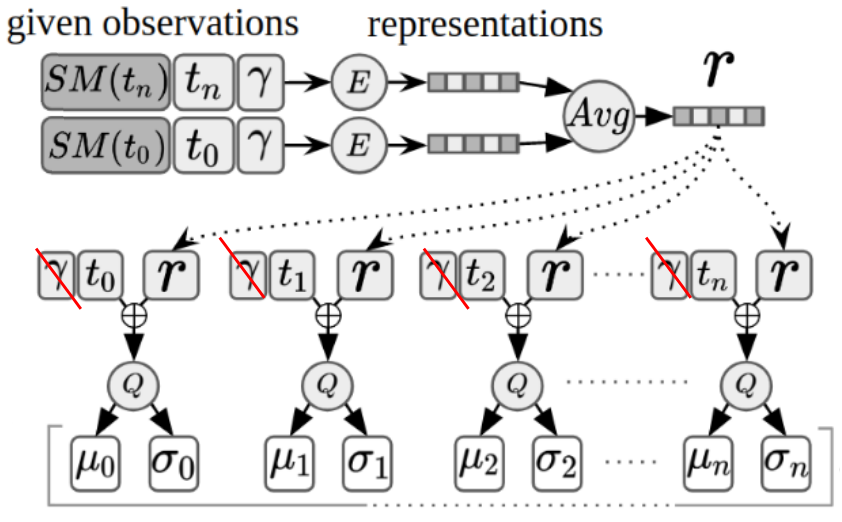
\includegraphics[width=0.7\linewidth]{figures/CNMP_short_no_tp_query.png}
    \caption{ Architecture of the CNMP model proposed without the original task parameter in the queries. }
    \label{fig:CNMP_short_no_tp_query}
\end{figure}

In \cref{fig:CNMP_short_no_tp_query}, the design changes can be compared to the original model. The neural network now feeds the decoder only with the time value to query and the constant representation of the conditions. As a result, the decoder has an input dimension less than the original model.

\begin{longtable}[c]{|c|l|c|c|}
\caption{Comparison Table of original CNMP vs CNMP with TP only in condition}
\label{tab:CNMPvsCNMPnoTPquery}\\
\hline
\textbf{MSE Error} & \textbf{TP} & \textbf{CNMP} & \textbf{CNMP TP condition} \\ \hline
\endfirsthead
\endhead
\multirow{2}{*}{\begin{tabular}[c]{@{}c@{}}on demonstrated\\ trajectory\end{tabular}} & 1 & 2.200240773631327e-06 & 0.0005239668753240399 \\ \cline{2-4} 
 & 2 & 2.852831969051669e-08 & 3.317327413240996e-05 \\ \hline
\multirow{2}{*}{\begin{tabular}[c]{@{}c@{}}on interpolated\\ trajectory\end{tabular}} & 1 & 2.8834989373212024e-06 & 0.0004749418782444545 \\ \cline{2-4} 
 & 2 & 2.598636844065303e-07 & 3.6395583963202646e-06 \\ \hline
\end{longtable}

The new model has been trained on the same dataset and verified with the same validation set.

The quantitative comparison results in \cref{tab:CNMPvsCNMPnoTPquery} show the average mean square errors (MSE) for every task on demonstrated trajectories and interpolated trajectories. The performance of the modified architecture exhibits an increase in the errors that, while present, is not significantly detrimental, suggesting a promising level of robustness in its overall functionality.

The qualitative results of the interpolation can be seen in \cref{fig:comparisonCNMPvsCNMPonlyTPcondition}, and although some interpolation differences are visible, they still clearly maintain a sufficient degree of correctness.

\begin{figure}
    \centering
    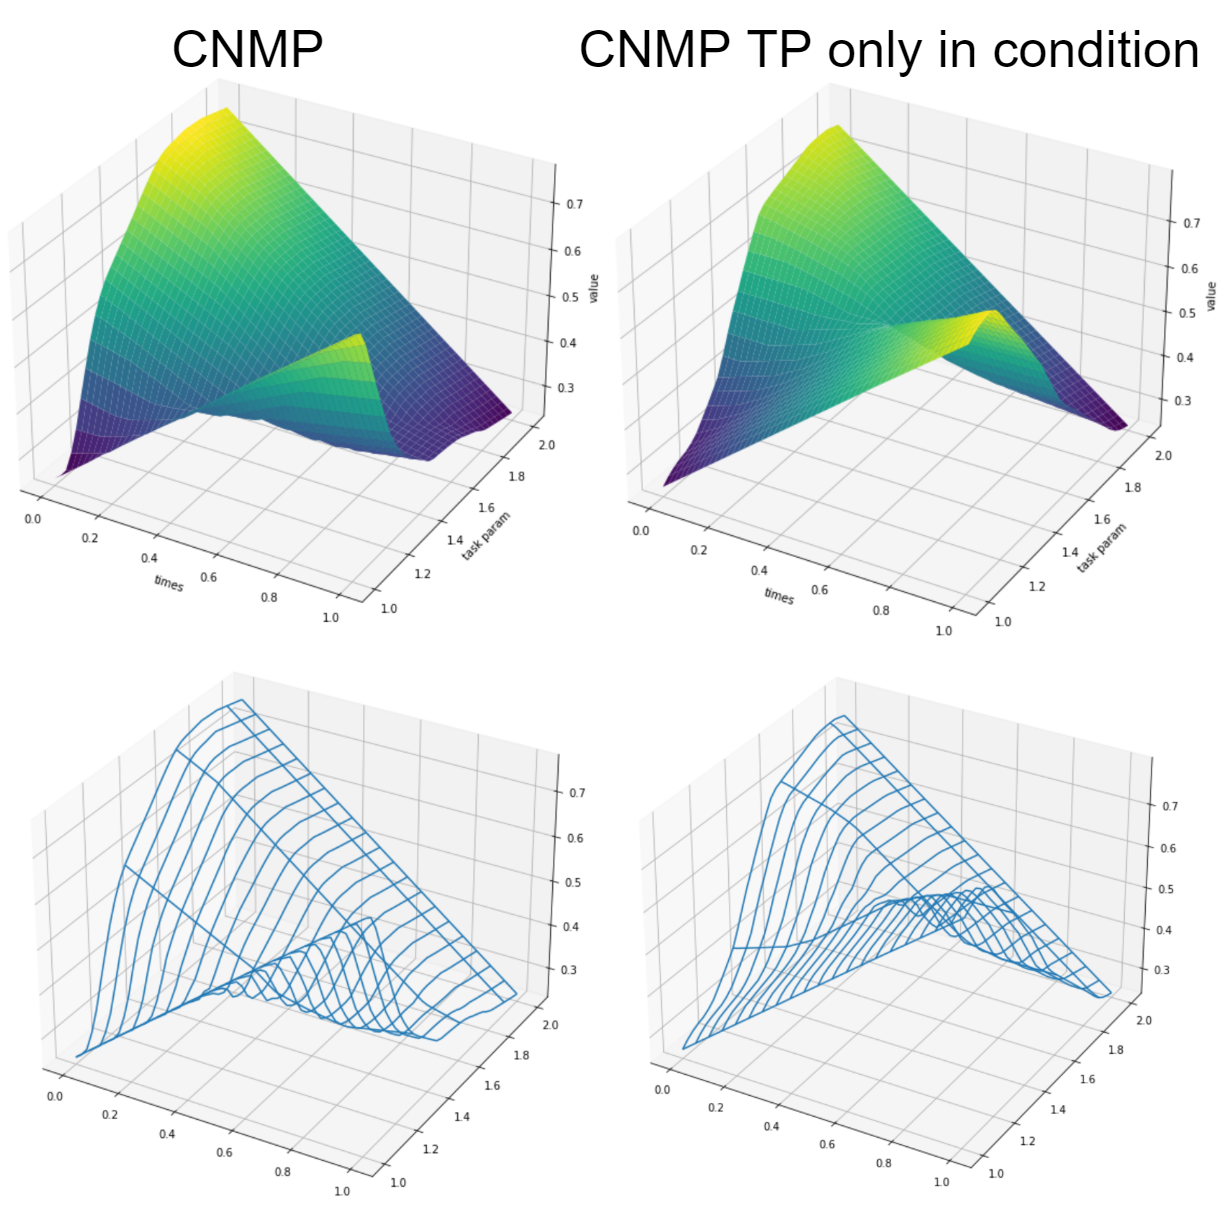
\includegraphics[width=0.8\linewidth]{figures/comparisonCNMPvsCNMPonlyTPcondition.png}
    \caption{ Interpolation comparison of CNMP model vs CNMP model with TP only in the condition. }
    \label{fig:comparisonCNMPvsCNMPonlyTPcondition}
\end{figure}



%%%%%% Network with only TP in query %%%%%%
\subsection{CNMP model with task-parameter only in query}
This subsection analyses the opposite alternative to the previous investigation. The architecture of the CNMP model is altered to generate the results using the task parameters (TPs) only in the input of the query. This design allows having conditioning points that are parameter-less and querying the network subsequently with the time $t$ and the task parameter $\gamma$. 

This architectural choice seems to be more appropriate for possible changes at run-time of skill by the model. However, it's clearly more challenging since the information is provided later in the pipeline. Moreover, conditioning points are responsible for the final position at every time $t$, and feeding the network only subsequently with the task forces it to infer the $\gamma$ of the conditions. 

\begin{figure}
    \centering
    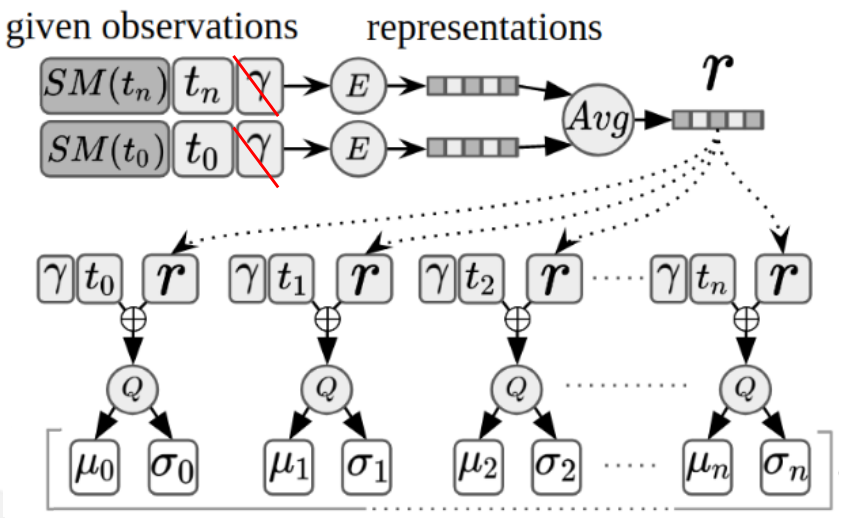
\includegraphics[width=0.7\linewidth]{figures/CNMP_short_no_tp_observations.png}
    \caption{ Architecture of the CNMP model proposed without the original task parameter in the observations. }
    \label{fig:CNMP_short_no_tp_observations}
\end{figure}

In \cref{fig:CNMP_short_no_tp_observations}, the design changes can be compared to the original model. The neural network now feeds the encoder with observations that don't have any parameter, delaying the $\gamma$ inference to the decoder. As a result, the encoder has an input dimension less than the original model.

\begin{longtable}[c]{|c|l|c|l|}
\caption{Comparison Table of original CNMP vs CNMP with TP only in query}
\label{tab:CNMPvsCNMPnoTPcondition}\\
\hline
\textbf{MSE Error} & \textbf{TP} & \textbf{CNMP} & \multicolumn{1}{c|}{\textbf{CNMP TP query}} \\ \hline
\endfirsthead
%
\endhead
%
\multirow{2}{*}{\begin{tabular}[c]{@{}c@{}}on demonstrated\\ trajectory\end{tabular}} & 1 & 2.200240773631327e-06 & 0.00015134105003480186 \\ \cline{2-4} 
 & 2 & 2.852831969051669e-08 & 1.5758800492775196e-05 \\ \hline
\multirow{2}{*}{\begin{tabular}[c]{@{}c@{}}on interpolated\\ trajectory\end{tabular}} & 1 & 2.8834989373212024e-06 & 0.0008166800702431865 \\ \cline{2-4} 
 & 2 & 2.598636844065303e-07 & 0.0002007523980230904 \\ \hline
\end{longtable}


The second new model has been trained on the same dataset and verified with the same validation set as the previously discussed ones.

The quantitative comparison results in \cref{tab:CNMPvsCNMPnoTPcondition} show the average mean square errors (MSE) for every task on demonstrated trajectories and interpolated trajectories. The modified architecture again demonstrates a rise in errors compared to the original model, but these errors, though now noticeable, do not compromise the usability of the model.

Not the same can be said for the qualitative results of the interpolation. The comparison that can be seen in \cref{fig:comparisonCNMPvsCNMPonlyTPquery} shows a remarkable drop in the values in the interpolated area between the two functions. This will clearly impact the correctness of a transition among them. The inaccuracy is probably due to the fact that the parameter information goes through an inferior network depth compared to the full model.  
Nevertheless, these results leave room for further research on how to condition with one state parameterless and let the network, queried with different tasks, pass through that state.

\begin{figure}
    \centering
    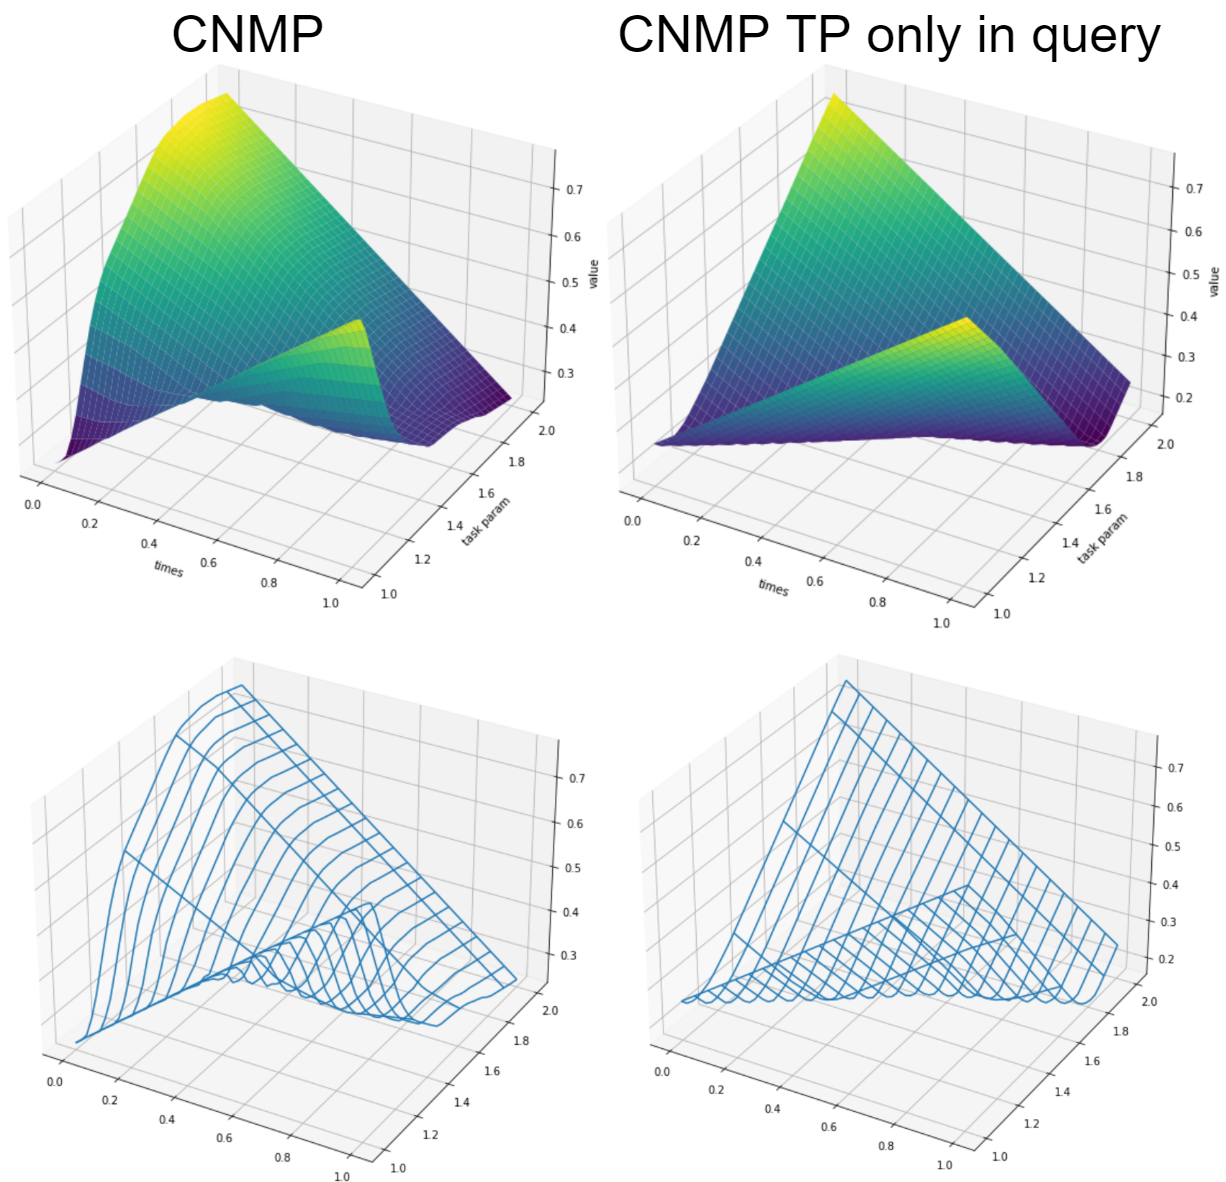
\includegraphics[width=0.8\linewidth]{figures/comparisonCNMPvsCNMPonlyTPquery.png}
    \caption{ Interpolation comparison of CNMP model vs CNMP model with TP only in the query. }
    \label{fig:comparisonCNMPvsCNMPonlyTPquery}
\end{figure}


%%%%%% Comparison %%%%%%
\subsection{Comparison of the previous models}
A comparison of the three previously discussed models is presented below to better evaluate the most capable and cross-validate the results. 
A different dataset was built with different parametric functions: linear, parabolic, and sinusoidal. This also implies the presence of three different tasks to feed to a single CNMP network. For each skill, different trajectories are present in the dataset to enable new trajectory generation for conditioning points of unseen values. 

Moreover, the transition among all tasks is now represented with three values, so the first task is encoded as $[1][0][0]$, the second as $[0][1][0]$, the third as $[0][0][1]$. This avoids passing through the middle one as in the case of a single parameter $[1..2..3]$ encoded network. The transition is performed by decreasing one value and increasing the other simultaneously.

\begin{longtable}[c]{|c|l|c|c|l|}
\caption{Full Comparison Table of errors of CNMP vs CNMP with TP only in condition vs CNMP with TP only in query}
\label{tab:CNMP3vs}\\
\hline
\textbf{\begin{tabular}[c]{@{}c@{}}MSE Error \\on \end{tabular}} & \textbf{TP} & \textbf{CNMP} & \textbf{\begin{tabular}[c]{@{}c@{}}CNMP \\ TP condition\end{tabular}} & \multicolumn{1}{c|}{\textbf{\begin{tabular}[c]{@{}c@{}}CNMP \\ TP query\end{tabular}}} \\ \hline
\endfirsthead
%
\endhead
%
\multirow{2}{*}{\begin{tabular}[c]{@{}c@{}}demonstrated\\ trajectory\end{tabular}} & 1 & 2.200240773e-06 & 0.0005239668753 & 0.00015134105003 \\ \cline{2-5} 
 & 2 & 2.852831969e-08 & 3.317327413e-05 & 1.5758800492e-05 \\ \hline
\multirow{2}{*}{\begin{tabular}[c]{@{}c@{}}interpolated\\ trajectory\end{tabular}} & 1 & 2.8834989373e-06 & 0.0004749418782 & 0.0008166800702 \\ \cline{2-5} 
 & 2 & 2.598636844e-07 & 3.6395583963e-06 & 0.0002007523980 \\ \hline
\end{longtable}

In \cref{fig:comparisonCNMP3trajectories}, it is possible to observe all the possible combinations for interpolating the different tasks on which the network has been trained. Even with more than two tasks and three dimensions added to the input the CNMP model performs sufficiently well in all three skills. 

\begin{figure}
    \centering
    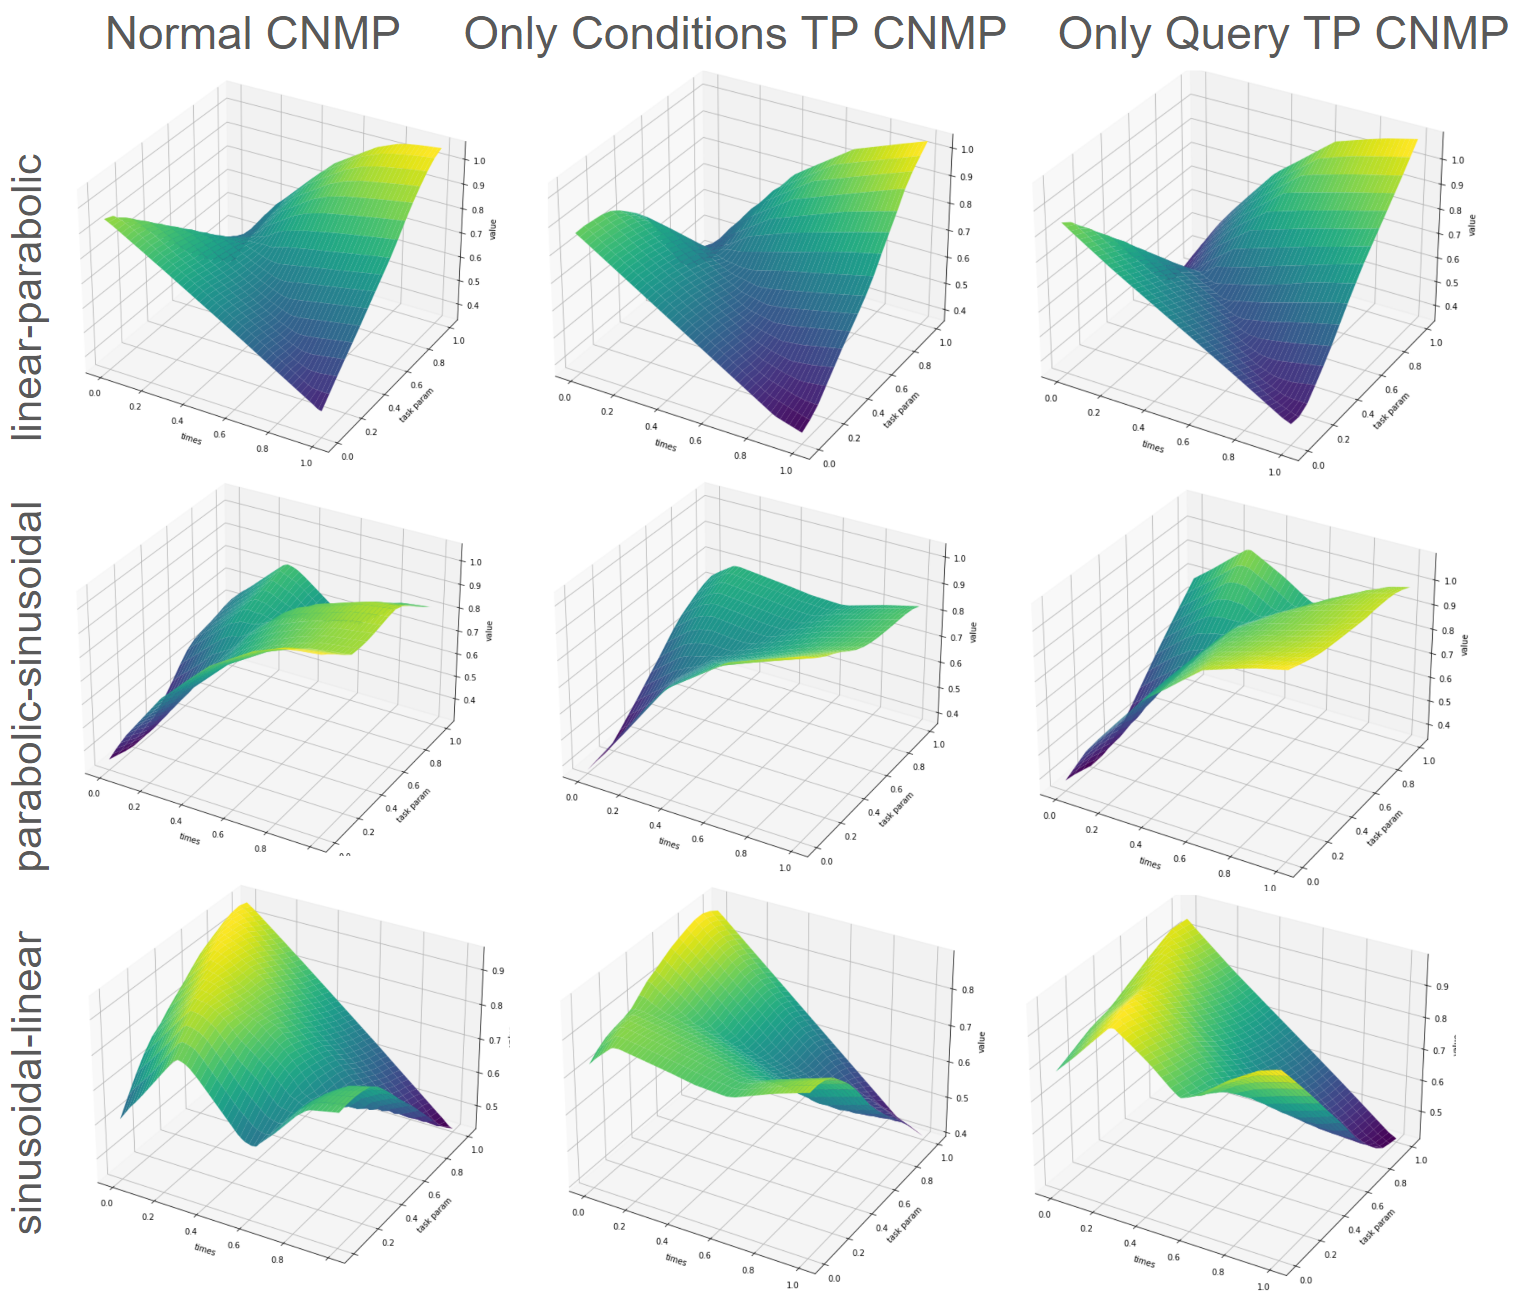
\includegraphics[width=0.9\linewidth]{figures/comparisonCNMP3trajectories.png}
    \caption{ Interpolation comparison of the 3 CNMP models analyzed for a different dataset and multiple tasks. }
    \label{fig:comparisonCNMP3trajectories}
\end{figure}


\newpage
%%%%%% shifting TP in time with 1 condition %%%%%%
\subsection{CNMP changing task in time with one conditioning point}
Analyzed the interpolation capabilities of the CNMP networks also on the task dimension, a possible method to shift the execution of a skill in time is proposed below. 

In order to build the interpolation visualizations, the network was always queried for every time-step with a constant $\gamma$. 
However, since the queries are independent, it's possible to query the time and parameter singularly as required.

Moreover, from the previously constructed plots, it is evident how it is possible to change tasks in time via querying the network with TPs linearly changing with time.

\begin{figure}
    \centering
    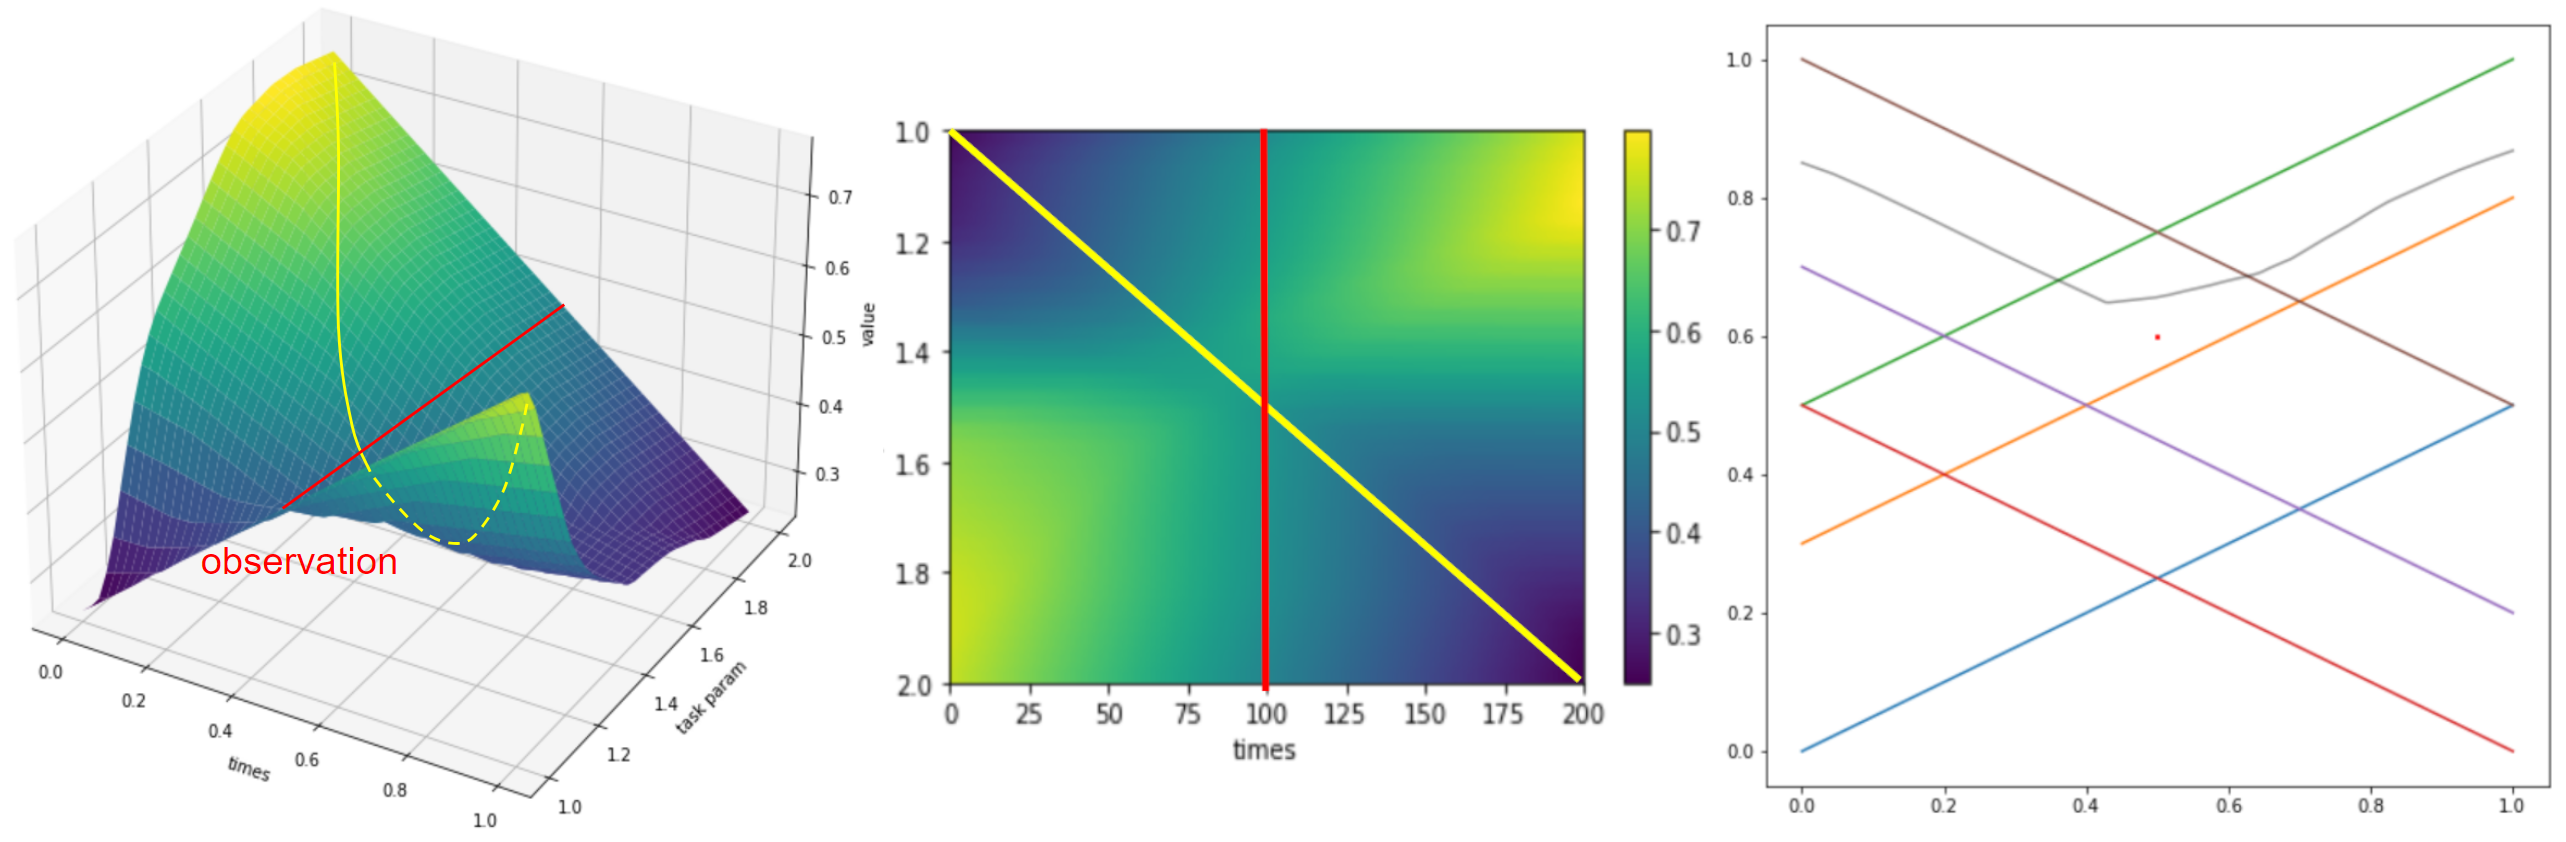
\includegraphics[width=0.95\linewidth]{figures/tpshift.png}
    \caption{ Transition in time of task through task parameter shifting }
    \label{fig:tpshift}
\end{figure}

In \cref{fig:tpshift}, the path of the queries of time and $\gamma$ is depicted in yellow. As time goes on, left to right, the action moves from descending (back of the graph) to ascending (front of the graph). This achieves a smooth change between task parameters using the interpolation space provided by the model. 

In this case, math leverages the neural network's hidden capabilities to wisely input the required parameters to generate the desired output. 

It's worth noting that this method works with any CNMP model variation previously discussed, as long as the interpolation space is built correctly. Further research could include better training to improve the results in the interpolation dimensions.  

The mixing of the two different skills is indeed performed through time, and in this case, the change is linear. Different functions analyzed produced different results, among them the most famous ones like sigmoid, logarithmic, and others. The model is capable of different transition speeds and periods depending on the selected function. The linear function is selected given that it produces the smoothest transitions since inclination is minimal in all the timesteps. 

On the opposite, a sharper function, like a step function in \cref{fig:tpshift-diff-functions}, produces a shift that is immediate and full-fledged a stitch among two parts. 

\begin{figure}
    \centering
    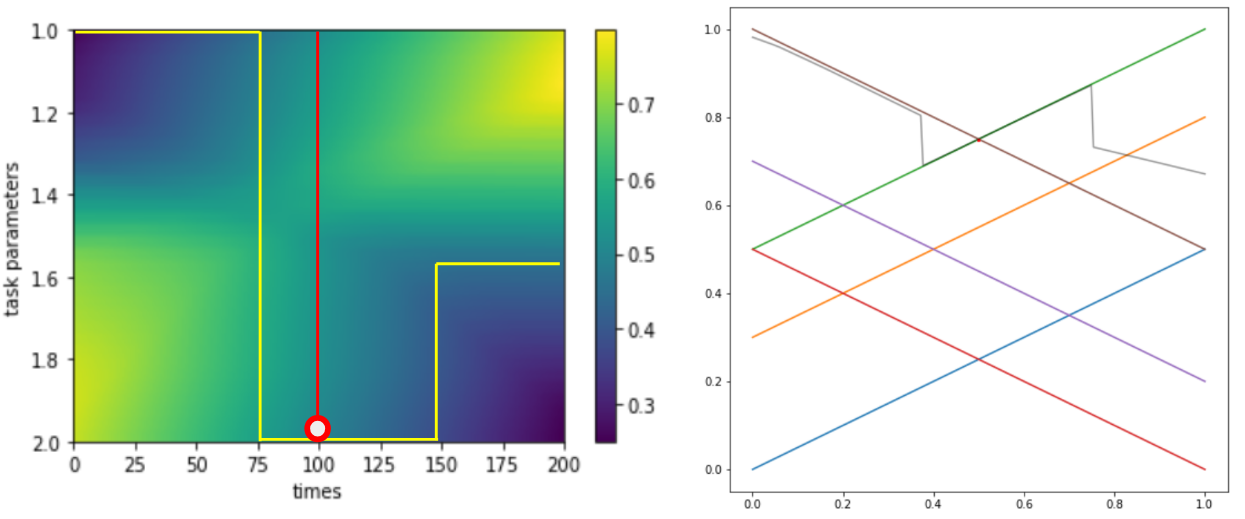
\includegraphics[width=0.8\linewidth]{figures/tpshift-diff-functions.png}
    \caption{ Different functions for changing task parameter in the CNMP network }
    \label{fig:tpshift-diff-functions}
\end{figure}

% 1 condition position discussion
In \cref{fig:tpshift}, it is possible to see that the final trajectory result is not passing through the conditioning point. This occurs since, at that moment $t=0.5$, the transition between two different task parameters is halfway ($\gamma=1.5$) and not fully on one $\gamma$. The interpolated space varies in quality depending on the network and its training, and this means the error would be higher compared to the values on $\gamma$ on which the model was trained. 

Surprisingly, it's not actually a problem because the conditioning point is nothing else than a point that symbolizes the transition between two conditioning points with different $\gamma$ located on different positions. The conditioning point is just a point that allows the transition without introducing any bias because it's part of both trajectories. In \cref{fig:tp-condition-point-meaning}, it is possible to see the red conditioning point emulating two different conditions with different TP, respectively descending for the left one and ascending for the right one.

This means that the conditioning point for transition is not meant to be anywhere, but it has to be at the intersection of the two desired functions with different TPs. This will grant the resulting function to pass at the initial time through the first conditioning point, since its TP is not mixed, and at the final time through the second condition for the same reason. 

In the example \cref{fig:tp-condition-point-meaning}, at time $t=0$, the function passes through the first point because the task parameter is fully descending. This is guaranteed because the red observation chosen is on the line produced by that initial point. In the same way, at time $t=1$, it's guaranteed to pass through the rightmost point because the observation is also on the function that is produced by that condition. 
For this reason, the observation point is not meant to be independent but derived from the two points to emulate.

\begin{figure}
    \centering
    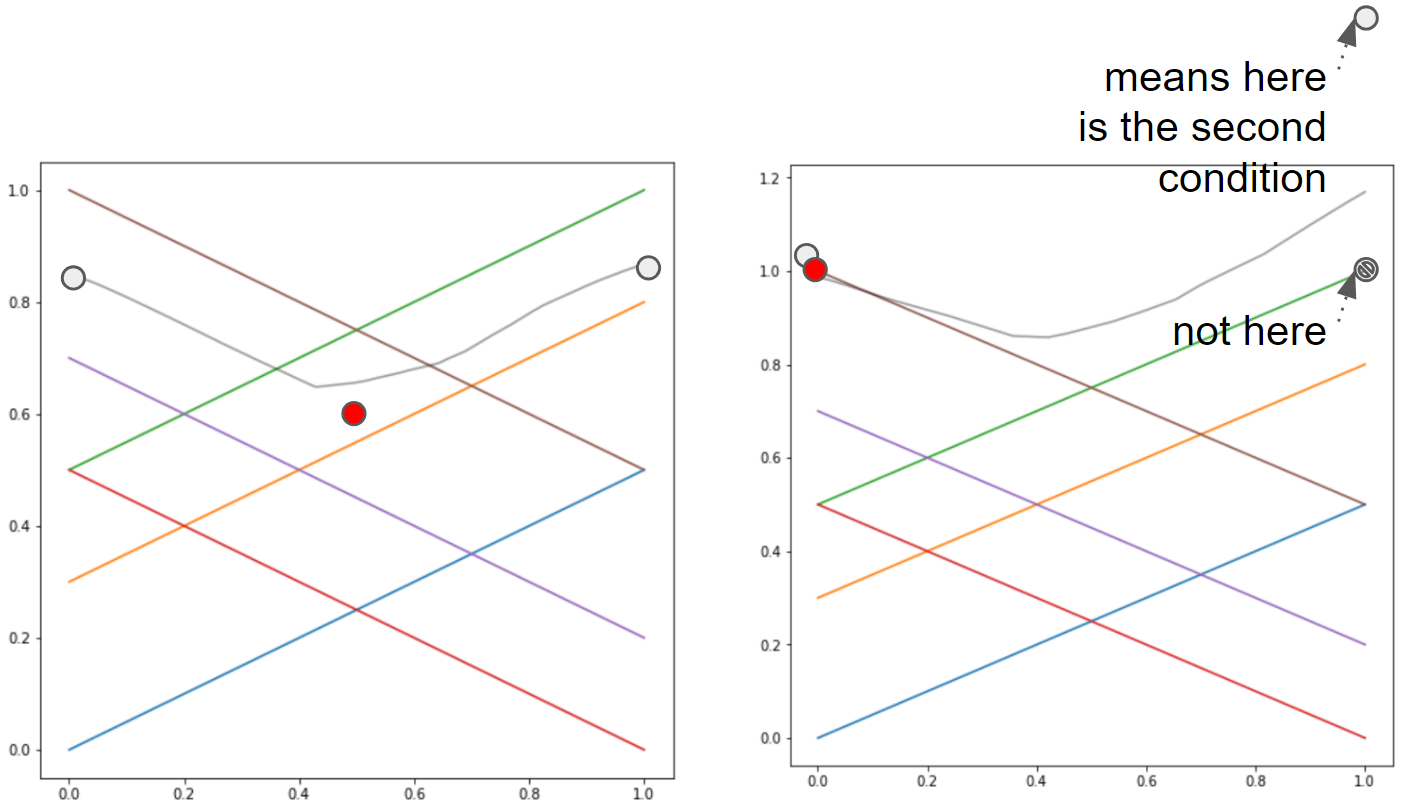
\includegraphics[width=0.8\linewidth]{figures/tp-condition-point-meaning.png}
    \caption{ A conditioning point that varies task parameter emulates two different conditioning points of different task parameters. }
    \label{fig:tp-condition-point-meaning}
\end{figure}

The best strategy to find the conditioning point for the transition among two conditions of different $\gamma$ seems to place it on the intersection of the two trajectories generated by these conditions. However, it is not always granted that the trajectories will intersect. As discussed above, in multidimensional spaces, the probability of this event decreases significantly. 

When two functions don't intersect, the best possible solution to not bias the interpolation is, while changing the $\gamma$, to shift as well the position of the condition in time. In the series of queries to the network, instead of giving the same context point and changing its task parameter, the position also changes. The optimal change of position is from a point on the first function generated by the first condition to the closest point on the function generated by the second condition. This guarantees the series of points will stay on the interpolation of the two functions and generate the desired interpolation surface area.

Extending the concept, the algorithm defined looks for the closest points among the two functions, and it transitions among them. 
The closest couple of points is looked only in the time span in which the network was trained, since it is a computation of cost $t^2$.
If there is an intersection, the change on the conditioning point will be only on the task parameter. 
If there is no intersection, the change of the conditioning point will also be a change in position from the closest point of the first function to the closest of the second one.


%%%%%% shifting TP in time with multiple conditions  %%%%%%
\subsection{CNMP changing task in time with multiple conditioning points}
The system developed enables a single transition using a single conditioning point. The shift occurs completely from an initial time that is $t=0$ to the final time of the network training.

It's a remarkable success because the bare normal CNMP model is completely incapable of changing the task coherently and continuously among its predictions. 
If fed with two conditions of different TP, the network outputs a completely unusable trajectory. This trajectory is a rough average of all the different ones generated by the conditioning points. This is due to the fact that the model, by definition, doesn't have an attention mechanism and doesn't lose the conditioning power in time.

However, this research extends the method further to multiple conditions with different task parameters. This enables the full control and customization of the predicted output. 

Furthermore, it achieves the shift among the observations in a desired time span not restricted to the full training time length. 

Once the interpolated surface is built, the time constraints are resolved with a fast transition from the first condition timestep to the second condition timestep. The resulting output sequence will still reside on the interpolated surface but, having less time, will be faster.

\begin{figure}
    \centering
    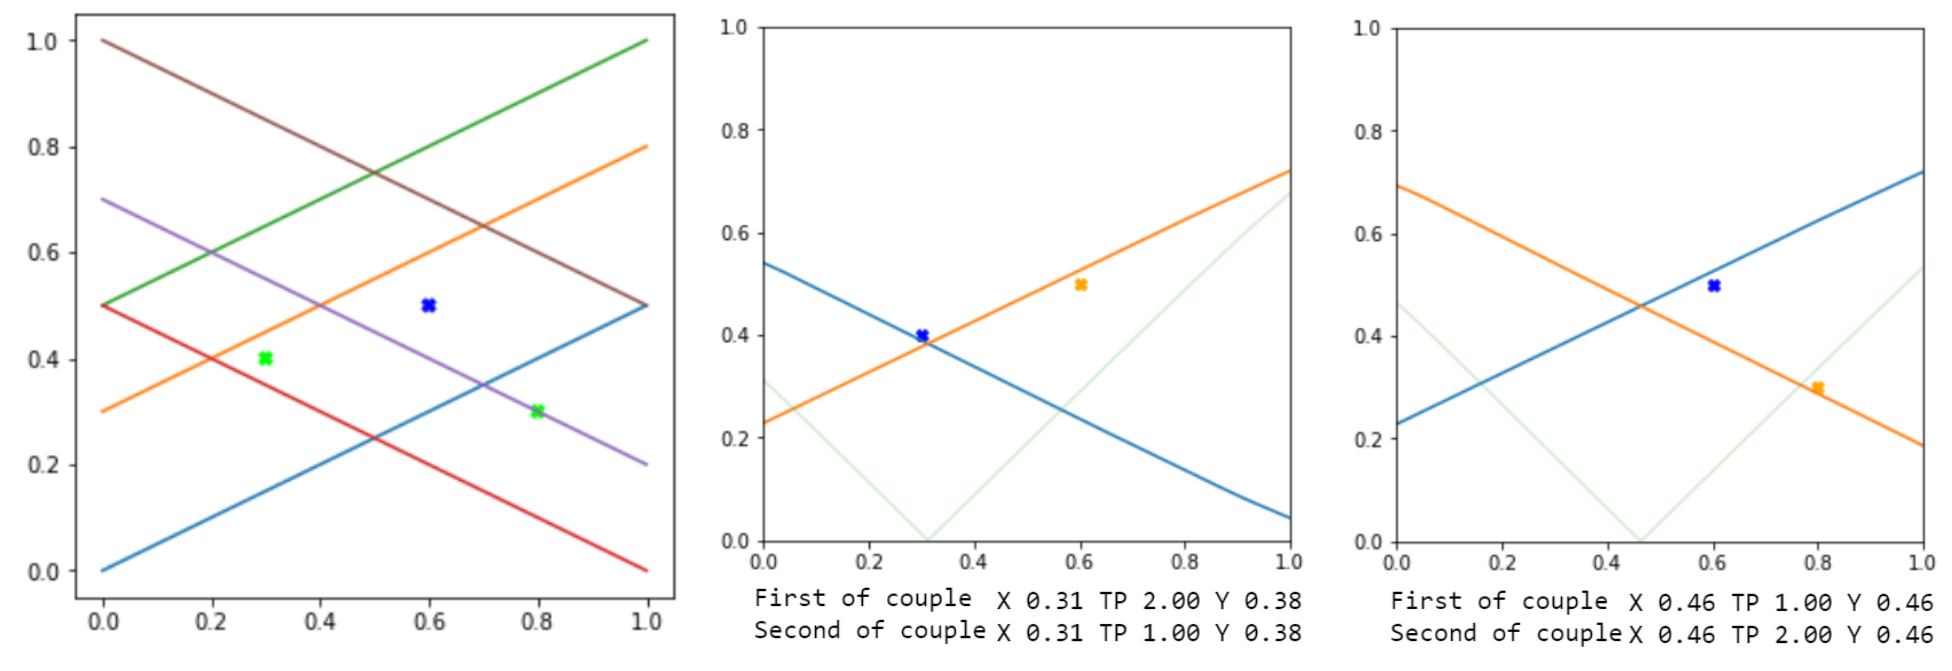
\includegraphics[width=0.95\linewidth]{figures/tp-multiple-shift.png}
    \caption{ Procedure to individuate multiple conditions for multiple shifts in the task parameters. }
    \label{fig:tp-multiple-shift}
\end{figure}

The multiple transitions are achieved by coupling them one by one in temporal order, so the first one determines the task parameter till its time. Then, between the first and the second one, the task is shifted. At the second observation, the task parameter will be fully on its task, but subsequently, will start to be merged with the third one, and so on. This guarantees that at the observation's times, the output function will pass through them, but in between, the task change will occur.  

In \cref{fig:tp-multiple-shift}, it is possible to view the initial observations of different parameters, two green conditioning points for the descending task and one blue in the middle for the ascending task. The first couple in temporal order is selected. At this point, the two functions each condition will independently create are generated. Those are visible in the \cref{fig:tp-multiple-shift} in the second plot. 

The closest points between these functions are selected, the absolute distance among the points is plotted as the green line at the bottom of the plot. In this case, since there is an intersection, the couple selected has the same starting and ending position, which only differs for the $\gamma$ parameter. During the shift time, the conditioning point of the network will transition from the first identified to the other one, changing TP. If the two closest points were in different locations, it would also change location, along with task parameter. 
The network is queried at the appropriate time with the condition designated.

\begin{figure}
    \centering
    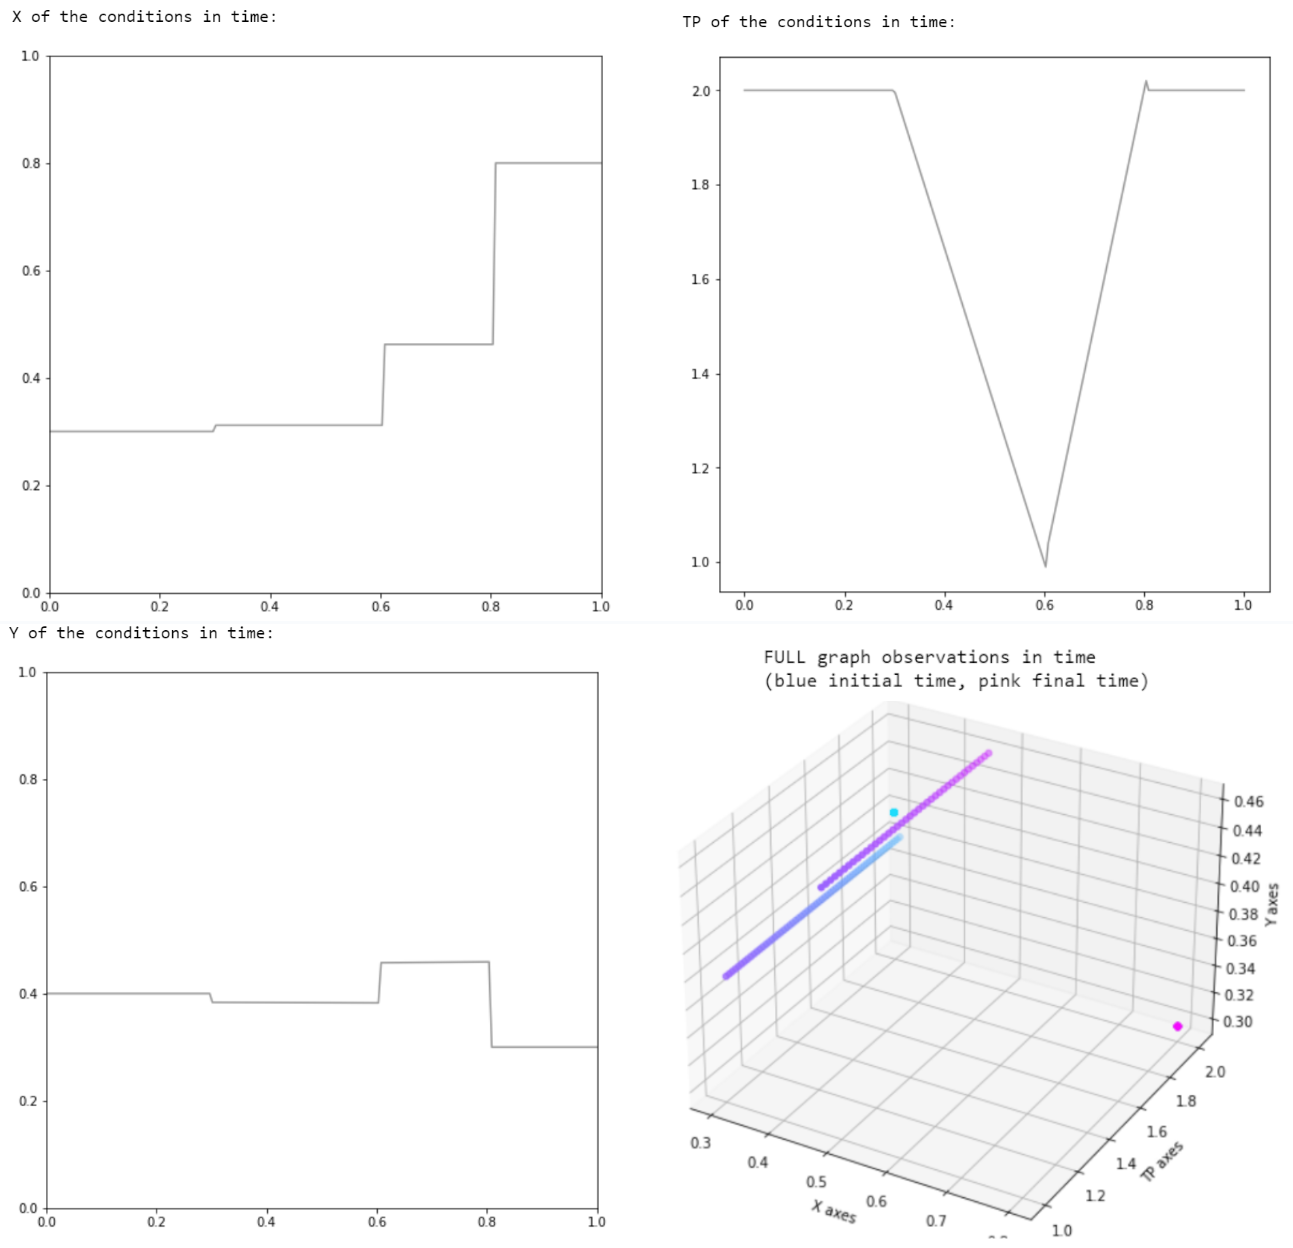
\includegraphics[width=0.7\linewidth]{figures/tp-multiple-shift-condition.png}
    \caption{ Graph and full path in time of the condition point used to transition multiple tasks parameters }
    \label{fig:tp-multiple-shift-condition}
\end{figure}


The process repeats for the second couple and so on to find the conditioning points to feed the network to obtain the desired result. 
The final full path of the conditioning point is visible in \cref{fig:tp-multiple-shift-condition} where it changes position in time according to the place where it will not bias the current transition. Meanwhile, the changing of the TP will occur during the time span designated.

It's worth noting that the conditioning point will also change its time, independently from the time queried. For this reason, in the 3D graph in \cref{fig:tp-multiple-shift-condition} the fourth dimension is introduced as color. The x axes of the graph corresponds now to the time of the condition, while the time of the queries corresponds to the change in color. 

Finally, the results shown in \cref{fig:tp-multiple-shift-results} demonstrate how this method can achieve trajectory predictions that are coherent across multiple shifts of tasks. The normal CNMP model with the same conditioning points is reported aside for comparison. 

\begin{figure}
    \centering
    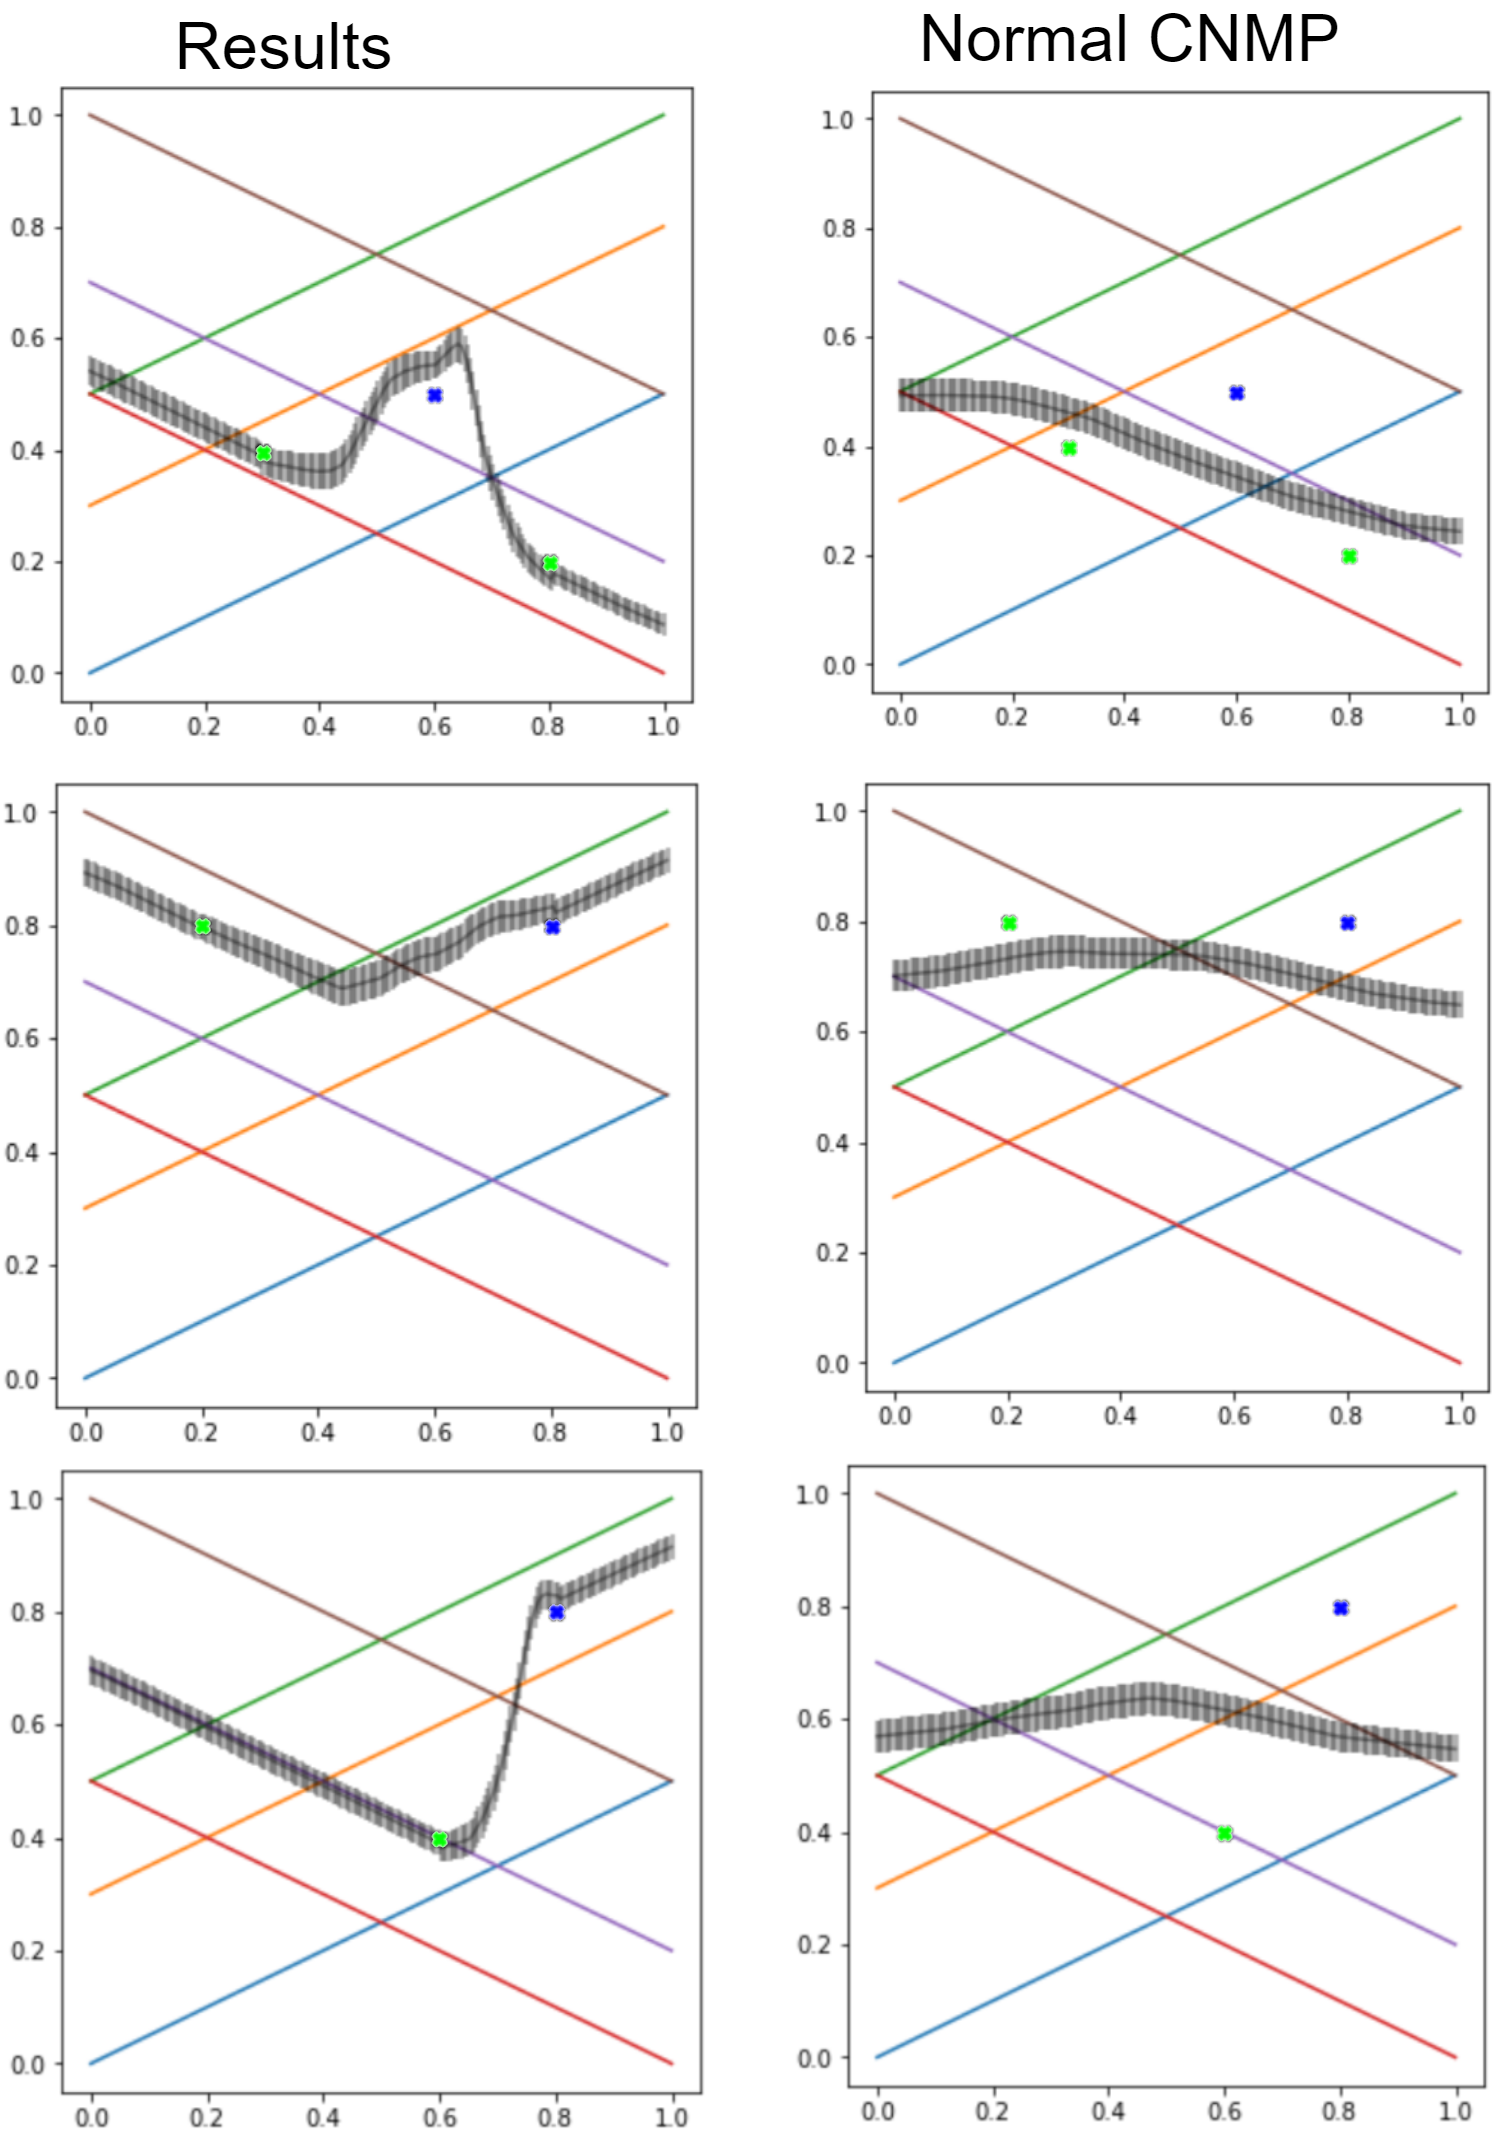
\includegraphics[width=0.9\linewidth]{figures/tp-multiple-shift-results.png}
    \caption{ Final results of multiple tasks transition and comparison with traditional CNMP network. }
    \label{fig:tp-multiple-shift-results}
\end{figure}


\newpage
%%%%%%%%%%%%%%%%%%%%%%%%%%%%%%%%%%%%%%%%%%%%%%%%
\section{End-To-End Skill Concatenation}
%%%%%%%%%%%%%%%%%%%%%%%%%%%%%%%%%%%%%%%%%%%%%%%%


    %----------------------------------------------------------------------------------------
\chapter{Implementation} 
\label{chap:implementation}
%----------------------------------------------------------------------------------------

Write implementation here.

\lstinputlisting[float,	language=Java, caption={A piece of code},	label={lst:pieceofcode}]{listings/HelloWorld.java}
You may need to reference listings in your thesis.
%
In this case, you are encouraged to make them \emph{floating}, and reference them by means of labels.
%
For instance, in \Cref{lst:pieceofcode}, we describe an hello world program in Java.

    %----------------------------------------------------------------------------------------
\chapter{Validation} % possible chapter for Projects
\label{chap:validation}
%----------------------------------------------------------------------------------------

Write implementation here
    %----------------------------------------------------------------------------------------
\chapter{Conclusions}
\label{chap:conclusions}
%----------------------------------------------------------------------------------------

Humans are capable of executing a wide variety of complex actions, based on prior experience. 
In this thesis, we provided a possible approach to novel high-level skill generation by combining movement primitives learned by CNMP models. 

\section{Future work}
Possible future works are ...

    
    %----------------------------------------------------------------------------------------
    % BIBLIOGRAPHY
    
    %\nocite{*} % uncomment this to show all the references in the .bib file
    \bibliographystyle{plain}
    \bibliography{References}
    
    %----------------------------------------------------------------------------------------

\end{document}